%%%%%%%%%%%%%%%%%%%%%%%%%%%%%%%%%%%%%%%%%%%%%%%%%%%%%%%%%%%%%%%%%%%%%%%%
%                                                                      %
%     File: Thesis_Methodology.tex                                     %
%     Tex Master: Thesis.tex                                           %
%                                                                      %
%%%%%%%%%%%%%%%%%%%%%%%%%%%%%%%%%%%%%%%%%%%%%%%%%%%%%%%%%%%%%%%%%%%%%%%%

\chapter{Proposed Methodology}
\label{chapter:methodology}

This chapter presents the theoretical and algorithmic methodology developed in this work for the autonomous cooperative control of the tethered USV-UAV system. It is structured into two main parts: Section~\ref{sec:system_modeling} derives the control-oriented kinematic and dynamic models of both vehicles, their actuator mappings, and the physical coupling introduced by the tether; Section~\ref{sec:system_control} then formulates the cooperative Nonlinear Model Predictive Control (NMPC) architecture that exploits these models to compute optimal, collision-free, and constraint-respecting trajectories.

%%%%%%%%%%%%%%%%%%%%%%%%%%%%%%%%%%%%%%%%%%%%%%%%%%%%%%%%%%%%%%%%%%%%%%%%
%                                                                      %
%     File: Methodology/01_SystemModeling.tex                          %
%     Tex Master: ../Thesis.tex                                        %
%                                                                      %
%%%%%%%%%%%%%%%%%%%%%%%%%%%%%%%%%%%%%%%%%%%%%%%%%%%%%%%%%%%%%%%%%%%%%%%%

\section{System Modeling}
\label{sec:system_modeling}
\label{chapter:modeling}

Real-time control needs models that are simple enough to compute quickly, yet detailed enough to capture how each vehicle actually moves and interacts with the other. The kinematics, dynamics, and physical coupling between the two vehicles let the controller predict how the system evolves and compute feasible, optimal trajectories.

The reference frames and notation are fixed first, followed by the kinematic and dynamic models of the \gls{usv} and the \gls{uav}.


% ==============================================================================
% SECTION 3.1: Reference Coordinate Frames and Notation
% ==============================================================================
\subsection{Reference Coordinate Frames and Notation}
\label{sec:mod_coordinates}

Deriving the equations of motion requires specifying the frames against which positions, orientations, and velocities are measured. Since the vessel and the drone move both with respect to the world and with respect to each other, a common frame of reference is required to describe their motion. Figure~\ref{fig:coordinate_frames} illustrates these frames.

\paragraph{Inertial Reference Frame $\{\mathcal{I}\}$}
This frame establishes the global coordinate system following the East-North-Up (ENU) convention, aligned with the standard ROS convention. Its origin $\mathcal{O}_I$ is fixed at an arbitrary point on the water surface within the operating area, following the usual flat-Earth convention. The axis $\mathbf{x}^{\mathcal{I}}$ points East, $\mathbf{y}^{\mathcal{I}}$ points North, and $\mathbf{z}^{\mathcal{I}}$ points upward, opposite to gravity.

\paragraph{USV Body-Fixed Reference Frame $\{\mathcal{B}_v\}$}
This frame is rigidly attached to the vessel, with origin $\mathcal{O}_v$ at its centre of gravity. This choice decouples the linear and rotational momentum equations. The forward-pointing axis $\mathbf{x}^{\mathcal{B}_v}$ defines surge, $\mathbf{y}^{\mathcal{B}_v}$ points to port (sway), and $\mathbf{z}^{\mathcal{B}_v}$ points upward (heave).

\paragraph{UAV Body-Fixed Reference Frame $\{\mathcal{B}_a\}$}
Similarly, this frame attaches to the UAV, with origin $\mathcal{O}_a$ at its centre of gravity, decoupling the translational and rotational dynamics in the same way. The longitudinal axis $\mathbf{x}^{\mathcal{B}_a}$ points forward, the lateral axis $\mathbf{y}^{\mathcal{B}_a}$ points to the left, and the vertical axis $\mathbf{z}^{\mathcal{B}_a}$ points upward, aligning with the collective thrust direction.

\begin{figure}[H]
    \centering
    % Colors: Okabe-Ito colorblind-safe qualitative palette (Okabe and Ito, 2008)
    \definecolor{okiBlue}{rgb}{0.0,0.447,0.698}       % Inertial frame {I}
    \definecolor{okiGreen}{rgb}{0.0,0.620,0.451}      % USV body frame {Bv}
    \definecolor{okiOrange}{rgb}{0.902,0.624,0.0}     % UAV body frame {Ba}
    \definecolor{okiVermillion}{rgb}{0.835,0.369,0.0} % Anchor / coupling point
    
    \begin{tikzpicture}[
        >=stealth,
        scale=1.0,
        axis/.style={->,okiBlue,thick,line width=1.2pt},
        bodyaxis/.style={->,okiGreen,thick,line width=1.2pt},
        uavaxis/.style={->,okiOrange,thick,line width=1.2pt},
        label/.style={black,font=\small},
        tether/.style={draw,line width=1.5pt,darkgray,smooth}
    ]
        % -- WATER SURFACE (z = 0) --
        \draw[black, dashed, line width=0.8pt] (-1.0,0) -- (10.0,0) node[right, font=\scriptsize, black!80] {Water Surface ($z^{\mathcal{I}}=0$)};

        % -- INERTIAL FRAME {I} --
        \coordinate (OI) at (0,0);
        \draw[axis] (OI) -- (2.0,0) node[below right,label,okiBlue] {$\mathbf{x}^{\mathcal{I}}$ (East)};
        \draw[axis] (OI) -- (1.0,0.8) node[above right,label,okiBlue] {$\mathbf{y}^{\mathcal{I}}$ (North)};
        \draw[axis] (OI) -- (0,2.0) node[above,label,okiBlue] {$\mathbf{z}^{\mathcal{I}}$ (Up)};
        \node[below left,label,okiBlue] at (OI) {$\{\mathcal{I}\}$};

        % -- USV FRAME {Bv} (Catamaran seen from the side, sitting at z=0) --
        \coordinate (Ov) at (5.5,0.45);
        \begin{scope}[shift={(Ov)}]
            % WAM-V pontoon (hull), side view
            \draw[thick,fill=gray!30] (-1.2,-0.45) -- (0.8,-0.45) to[out=0,in=-120] (1.3,-0.15) -- (-1.2,-0.15) -- cycle;
            % Support arch legs
            \draw[line width=1.5pt,black] (-0.6,-0.15) -- (-0.3,0.3);
            \draw[line width=1.5pt,black] (0.6,-0.15) -- (0.3,0.3);
            % Upper deck
            \draw[thick,fill=gray!50] (-0.5,0.3) rectangle (0.5,0.45);
            
            % Boat body axes (side/3D view)
            \draw[bodyaxis] (0,0) -- (1.8,0) node[right,label,okiGreen] {$\mathbf{x}^{\mathcal{B}_v}$};
            \draw[bodyaxis] (0,0) -- (0,1.5) node[right,label,okiGreen,xshift=2pt,yshift=-4pt] {$\mathbf{z}^{\mathcal{B}_v}$};
            \draw[bodyaxis] (0,0) -- (0.6,0.48) node[above,label,okiGreen,xshift=-3pt] {$\mathbf{y}^{\mathcal{B}_v}$};
            
            % Anchor point, vertically aligned with the CG
            \coordinate (Pa) at (0,0.45);
            \fill[white] (Pa) circle (4pt); % break the z_v arrow shaft behind the marker
            \fill[okiVermillion] (Pa) circle (2.5pt) node[above left,font=\scriptsize,black] {Anchor};
        \end{scope}

        \node[below,label,okiGreen] at ($(Ov)+(0,-0.45)$) {$\{\mathcal{B}_v\}$};

        % -- UAV FRAME {Ba} (Drone seen from the side/front, flying in 3D with pitch tilt) --
        \coordinate (Oa) at (9.0,3.5);
        \begin{scope}[shift={(Oa)}, rotate=-15]
            % Drone cross arms in 3D (side/isometric perspective)
            \draw[thick,line width=1.5pt,black] (-0.6,-0.15) -- (0.6,0.15);
            \draw[thick,line width=1.5pt,black] (-0.5,0.15) -- (0.5,-0.15);
            % Central body
            \fill[black] (0,0) circle (3.5pt);
            % The 4 rotors/propellers at the arm tips
            \draw[gray, thin] (-0.6,-0.1) ellipse (3pt and 0.8pt);
            \draw[gray, thin] (0.6,0.2) ellipse (3pt and 0.8pt);
            \draw[gray, thin] (-0.5,0.2) ellipse (3pt and 0.8pt);
            \draw[gray, thin] (0.5,-0.1) ellipse (3pt and 0.8pt);
            
            % Drone body axes (tilt with the vehicle body)
            \draw[uavaxis] (0,0) -- (1.4,0) node[right,label,okiOrange] {$\mathbf{x}^{\mathcal{B}_a}$};
            \draw[uavaxis] (0,0) -- (0,1.4) node[above,label,okiOrange] {$\mathbf{z}^{\mathcal{B}_a}$};
            \draw[uavaxis] (0,0) -- (0.5,0.4) node[above right,label,okiOrange] {$\mathbf{y}^{\mathcal{B}_a}$};
        \end{scope}
        
        \node[below,label,okiOrange] at ($(Oa)+(0,-0.50)$) {$\{\mathcal{B}_a\}$};

        % -- TETHER --
        % Smooth curve representing the tether, labeled below right to avoid overlaps with the axes
        \draw[tether] (Pa) .. controls ($(Pa)+(1.5,-0.2)$) and ($(Oa)+(-1.0,-1.0)$) .. (Oa);
        \path (Pa) .. controls ($(Pa)+(1.5,-0.2)$) and ($(Oa)+(-1.0,-1.0)$) .. (Oa);

    \end{tikzpicture}
    \caption{Reference coordinate frames $\{\mathcal{I}\}$, $\{\mathcal{B}_v\}$, and $\{\mathcal{B}_a\}$.}
    \label{fig:coordinate_frames}
\end{figure}

% ==============================================================================
% SECTION 3.2: WAM-V Surface Vessel Model
% ==============================================================================
\subsection{WAM-V Surface Vessel Model}
\label{sec:mod_usv}

The mathematical model of the WAM-V catamaran, covering its horizontal maneuvering dynamics and thruster allocation, forms a control-oriented state-space model suitable for trajectory tracking and predictive control.

Although a rigid body moving freely in the marine environment inherently has six degrees of freedom, the WAM-V is a vessel that moves on the surface, which allows the motion to be simplified to the horizontal plane. Under this assumption, the model is reduced to three degrees of freedom.

Predicting the vessel's motion, as needed for trajectory tracking and predictive control, requires knowing how its state changes over time for a given input. This relationship is captured by the nonlinear state-space model
\begin{equation}
    \label{eq:usv_state_space_generic}
    \dot{\mathbf{x}}_v = f(\mathbf{x}_v, \mathbf{u}_v),
\end{equation}
The state vector $\mathbf{x}_v \in \mathbb{R}^6$ is given by
\begin{equation}
    \label{eq:usv_state_vector}
    \mathbf{x}_v = [x, y, \psi, u, v, r]^\top,
\end{equation}
where:
\begin{itemize}
    \item $x, y$ -- position of the origin $\mathcal{O}_v$ of $\{\mathcal{B}_v\}$ relative to $\{\mathcal{I}\}$, expressed in $\{\mathcal{I}\}$;
    \item $\psi$ -- heading of $\{\mathcal{B}_v\}$ relative to $\{\mathcal{I}\}$;
    \item $u, v$ -- surge and sway linear velocities of $\{\mathcal{B}_v\}$ relative to $\{\mathcal{I}\}$, expressed in $\{\mathcal{B}_v\}$;
    \item $r$ -- angular velocity of $\{\mathcal{B}_v\}$ relative to $\{\mathcal{I}\}$, expressed in $\{\mathcal{B}_v\}$;
\end{itemize}
The control input vector $\mathbf{u}_v \in \mathbb{R}^3$ is given by
\begin{equation}
    \label{eq:usv_input_vector}
    \mathbf{u}_v = [X, Y, N]^\top,
\end{equation}
where:
\begin{itemize}
    \item $X$ -- surge force generated by the propulsion system, applied to $\{\mathcal{B}_v\}$, expressed in $\{\mathcal{B}_v\}$;
    \item $Y$ -- sway force generated by the propulsion system, applied to $\{\mathcal{B}_v\}$, expressed in $\{\mathcal{B}_v\}$;
    \item $N$ -- yaw moment generated by the propulsion system, applied to $\{\mathcal{B}_v\}$, expressed in $\{\mathcal{B}_v\}$;
\end{itemize}
The vector field $f(\cdot)$ splits into a kinematic block and a dynamic block, derived in turn in the following subsections.

\subsubsection{Kinematic Model}
\label{subsec:mod_usv_kinematics}
The kinematics describe how the vessel's inertial position and heading evolve as a function of its body-fixed velocities, forming the first half of \eqref{eq:usv_state_space_generic}.

Let $\mathbf{p} = x\,\mathbf{x}^{\mathcal{I}} + y\,\mathbf{y}^{\mathcal{I}}$ denote the inertial position of the origin $\mathcal{O}_v$ of $\{\mathcal{B}_v\}$. Since $\mathbf{x}^{\mathcal{I}}, \mathbf{y}^{\mathcal{I}}$ are constant, differentiating yields
\begin{equation}
    \dot{\mathbf{p}} = \dot{x}\,\mathbf{x}^{\mathcal{I}} + \dot{y}\,\mathbf{y}^{\mathcal{I}},
    \label{eq:usv_pdot_inertial_def}
\end{equation}
i.e.\ $\dot{x}, \dot{y}$ are, by definition, the components of $\dot{\mathbf{p}}$ in the inertial frame.

The surge and sway velocities $u, v$ are defined in the body-fixed frame, so that
\begin{equation}
    \dot{\mathbf{p}} = u\,\mathbf{x}^{\mathcal{B}} + v\,\mathbf{y}^{\mathcal{B}},
    \label{eq:usv_pdot_body_frame}
\end{equation}
where $\mathbf{x}^{\mathcal{B}}, \mathbf{y}^{\mathcal{B}}$ denote the basis vectors of $\{\mathcal{B}_v\}$, i.e.\ $\mathbf{x}^{\mathcal{B}_v}, \mathbf{y}^{\mathcal{B}_v}$.

Since $\{\mathcal{B}_v\}$ is rotated relative to $\{\mathcal{I}\}$ by the heading angle $\psi$, the inertial unit vectors are related to the body-fixed ones by the rotation matrix $\mathbf{R}(\psi) \in SO(2)$,
\begin{equation}
    \begin{bmatrix} \mathbf{x}^{\mathcal{I}} \\ \mathbf{y}^{\mathcal{I}} \end{bmatrix} = \mathbf{R}(\psi) \begin{bmatrix} \mathbf{x}^{\mathcal{B}} \\ \mathbf{y}^{\mathcal{B}} \end{bmatrix},
    \label{eq:usv_basis_matrix}
\end{equation}
following the standard planar rotation matrix,
\begin{equation}
    \mathbf{R}(\psi) = \begin{bmatrix} \cos\psi & -\sin\psi \\ \sin\psi & \cos\psi \end{bmatrix},
    \label{eq:usv_rotation_matrix}
\end{equation}
which is equivalent to
\begin{equation}
    \mathbf{x}^{\mathcal{B}} = \cos\psi\,\mathbf{x}^{\mathcal{I}} + \sin\psi\,\mathbf{y}^{\mathcal{I}}, \qquad
    \mathbf{y}^{\mathcal{B}} = -\sin\psi\,\mathbf{x}^{\mathcal{I}} + \cos\psi\,\mathbf{y}^{\mathcal{I}}.
    \label{eq:usv_basis_change}
\end{equation}

Substituting \eqref{eq:usv_basis_change} into \eqref{eq:usv_pdot_body_frame} and grouping terms gives
\begin{equation}
    \dot{\mathbf{p}} = \underbrace{(u\cos\psi - v\sin\psi)}_{\dot{x}}\,\mathbf{x}^{\mathcal{I}} + \underbrace{(u\sin\psi + v\cos\psi)}_{\dot{y}}\,\mathbf{y}^{\mathcal{I}}.
    \label{eq:usv_pdot_expanded}
\end{equation}
Comparing with \eqref{eq:usv_pdot_inertial_def} then directly gives
\begin{equation}
    \dot{x} = u\cos\psi - v\sin\psi, \qquad \dot{y} = u\sin\psi + v\cos\psi,
\end{equation}
which is precisely
\begin{equation}
    \label{eq:usv_kinematics_planar}
    \begin{bmatrix} \dot{x} \\ \dot{y} \end{bmatrix} = \mathbf{R}(\psi)\begin{bmatrix} u \\ v \end{bmatrix}.
\end{equation}

The heading rate follows directly from the definition of the angular velocity $r$:
\begin{equation}
    \dot{\psi} = r. \label{eq:usv_psi_dot}
\end{equation}

\subsubsection{Dynamic Model}
\label{subsec:mod_usv_dynamics}

The dynamics describe how the vessel's body-fixed velocities evolve as a function of the applied forces and moments, forming the second half of \eqref{eq:usv_state_space_generic}.

Unlike $\mathbf{x}^{\mathcal{I}}, \mathbf{y}^{\mathcal{I}}$, the body-fixed unit vectors $\mathbf{x}^{\mathcal{B}}, \mathbf{y}^{\mathcal{B}}$ rotate with the vehicle. Differentiating \eqref{eq:usv_basis_change} and using $\dot\psi = r$ gives
\begin{equation}
    \dot{\mathbf{x}}^{\mathcal{B}} = r\,\mathbf{y}^{\mathcal{B}}, \qquad \dot{\mathbf{y}}^{\mathcal{B}} = -r\,\mathbf{x}^{\mathcal{B}}.
    \label{eq:usv_basis_dot}
\end{equation}
The inertial velocity, expressed in the body-fixed frame, is $\dot{\mathbf{p}} = u\,\mathbf{x}^{\mathcal{B}} + v\,\mathbf{y}^{\mathcal{B}}$. Differentiating once more and substituting \eqref{eq:usv_basis_dot} yields the inertial acceleration
\begin{equation}
    \ddot{\mathbf{p}} = (\dot{u} - vr)\,\mathbf{x}^{\mathcal{B}} + (\dot{v} + ur)\,\mathbf{y}^{\mathcal{B}},
    \label{eq:usv_pddot_body_frame}
\end{equation}
where the cross terms $-vr$ and $ur$ are Coriolis/centripetal terms arising because $\{\mathcal{B}_v\}$ is a rotating, non-inertial frame.

Let $F_x, F_y$ denote the resultant surge and sway forces applied at $\mathcal{O}_v$, so that $\mathbf{F} = F_x\,\mathbf{x}^{\mathcal{B}} + F_y\,\mathbf{y}^{\mathcal{B}}$. By Newton's second law, $\mathbf{F} = m\,\ddot{\mathbf{p}}$, and comparing with \eqref{eq:usv_pddot_body_frame},
\begin{equation}
    F_x = m(\dot{u} - vr), \qquad F_y = m(\dot{v} + ur).
    \label{eq:usv_newton_linear}
\end{equation}
Since the vessel's motion is planar, Euler's rotational equation about $\mathbf{z}^{\mathcal{B}}$ takes the form
\begin{equation}
    M_z = I_z\,\dot{r},
    \label{eq:usv_euler_yaw}
\end{equation}
where $M_z$ is the resultant yaw moment about $\mathcal{O}_v$ and $I_z$ the yaw moment of inertia.

The resultant force and moment $F_x, F_y, M_z$ combine two contributions: the thrust generated by the propulsion system, $X, Y, N$, and the hydrodynamic damping opposing the vessel's motion. This damping follows the standard linear-plus-quadratic model for surface vessels~\cite{fossenHandbookMarineCraft2011}. The quadratic surge term is further split into forward and backward coefficients, to capture the asymmetric drag between the two directions:
\begin{equation}
    F_x = X - \big(X_u + X_{uu}^{\pm}|u|\big)u, \qquad
    X_{uu}^{\pm} = \begin{cases} X_{uu}^{+}, & u \geq 0 \\ X_{uu}^{-}, & u < 0 \end{cases}
    \label{eq:usv_damping_surge}
\end{equation}
\begin{equation}
    F_y = Y - \big(Y_v + Y_{vv}|v|\big)v, \qquad
    M_z = N - \big(N_r + N_{rr}|r|\big)r.
    \label{eq:usv_damping_sway_yaw}
\end{equation}

Substituting \eqref{eq:usv_damping_surge}--\eqref{eq:usv_damping_sway_yaw} into \eqref{eq:usv_newton_linear} and \eqref{eq:usv_euler_yaw}, and solving for the accelerations, gives the dynamic block of \eqref{eq:usv_state_space_generic}:
\begin{equation}
    \dot{u} = \frac{1}{m}\Big[X - \big(X_u + X_{uu}^{\pm}|u|\big)u\Big] + vr,
    \label{eq:usv_udot}
\end{equation}
\begin{equation}
    \dot{v} = \frac{1}{m}\Big[Y - \big(Y_v + Y_{vv}|v|\big)v\Big] - ur,
    \label{eq:usv_vdot}
\end{equation}
\begin{equation}
    \dot{r} = \frac{1}{I_z}\Big[N - \big(N_r + N_{rr}|r|\big)r\Big].
    \label{eq:usv_rdot}
\end{equation}

\subsubsection{Thruster Allocation}
\label{subsec:mod_usv_thruster_allocation}

The thruster allocation maps the physical actuator commands, the left and right thrust magnitudes $T_L, T_R$ and azimuth angles $\alpha_L, \alpha_R$, to the resultant force and moment $X, Y, N$ required by the dynamics of Section~\ref{subsec:mod_usv_dynamics}, according to the geometry shown in Figure~\ref{fig:usv_planar_model}.

\begin{figure}[H]
    \centering
    % Colors: Okabe-Ito colorblind-safe qualitative palette. Body axes stay neutral
    % gray so color draws the eye to the forces, the physically meaningful content.
    \definecolor{okiBlue}{rgb}{0.0,0.447,0.698}       % Resultant control forces X, Y, N
    \definecolor{okiVermillion}{rgb}{0.835,0.369,0.0} % Raw thruster forces T_L, T_R
    
    \begin{tikzpicture}[
        >=stealth,
        scale=1.45,
        every node/.style={font=\small},
        axisV/.style={->, black!60, line width=1.3pt},
        forceVec/.style={->, okiVermillion, line width=1.4pt},
        resForce/.style={->, okiBlue, line width=1.3pt},
        dimLine/.style={<->, >=stealth, black!75, line width=0.6pt, font=\footnotesize},
        guideLine/.style={dashed, black!35, line width=0.5pt}
    ]
        % Geometrical Parameters
        \def\xarm{-2.6}
        \def\yarm{1.6}
        \def\alphaL{28}
        \def\alphaR{-22}

        % -- CATAMARAN CROSSBEAMS & DECK --
        % Connecting crossbeams between pontoons
        \draw[fill=gray!40, draw=black!70, line width=0.8pt] 
            (-1.4, -1.6) rectangle (-1.0, 1.6);
        \draw[fill=gray!40, draw=black!70, line width=0.8pt] 
            (0.6, -1.6) rectangle (1.0, 1.6);

        % Central Deck (with clean margins from pontoons)
        \draw[fill=gray!15, draw=black!65, line width=0.85pt, rounded corners=3pt] 
            (-1.5, -1.0) rectangle (1.1, 1.0);

        % Left Pontoon (Port)
        \draw[fill=gray!25, draw=black!85, line width=1.0pt, rounded corners=2pt]
            (-2.7, 1.35) -- (1.5, 1.35) -- (2.8, 1.6) -- (1.5, 1.85) -- (-2.7, 1.85) -- cycle;
        % Label shifted forward to avoid the y-axis at x=0
        \node[font=\scriptsize, black!65] at (0.8, 1.6) {Port Pontoon};

        % Right Pontoon (Starboard)
        \draw[fill=gray!25, draw=black!85, line width=1.0pt, rounded corners=2pt]
            (-2.7, -1.85) -- (1.5, -1.85) -- (2.8, -1.6) -- (1.5, -1.35) -- (-2.7, -1.35) -- cycle;
        % Label shifted forward to avoid the dimension guideline at x=0
        \node[font=\scriptsize, black!65] at (0.8, -1.6) {Starboard Pontoon};

        % Longitudinal Centerline
        \draw[guideLine] (-3.6, 0) -- (3.6, 0);

        % -- CENTER OF GRAVITY (CG) & BODY AXES --
        \fill[black] (0,0) circle (2.5pt);
        \draw[line width=0.7pt, black] (0,0) circle (5.0pt);
        \node[below left, font=\scriptsize, black, xshift=-4pt, yshift=-7pt] at (0,0) {$\mathcal{O}_v$ (CG)};

        % Body axes {Bv}
        \draw[axisV] (0,0) -- (3.6, 0) node[right, black!60] {$\mathbf{x}^{\mathcal{B}_v}$ (surge, $u$)};
        \draw[axisV] (0,0) -- (0, 2.7) node[above, black!60] {$\mathbf{y}^{\mathcal{B}_v}$ (sway, $v$)};
        
        % Yaw rate r (curved orange arrow in Quadrant I: R=0.65, 15° to 80°, span 65°)
        \draw[->, line width=1.1pt, black!60] (0.628, 0.168) arc (15:80:0.65) 
            node[above right, font=\small, black!60, xshift=-1pt, yshift=1pt] {$r$};

        % Resultant Control Forces at CG (X, Y, N) in MATLAB Blue
        \draw[resForce] (0,0) -- (1.5, 0) 
            node[above, font=\footnotesize, okiBlue, xshift=-2pt, yshift=2pt] {$X$};
        \draw[resForce] (0,0) -- (0, 1.4);
        % Y placed cleanly in the gap between deck (y=1.0) and pontoon (y=1.35)
        \node[left, font=\footnotesize, okiBlue, xshift=-2pt] at (0, 1.18) {$Y$};
        % Moment N in Quadrant II (identically sized: R=0.65, 115° to 180°, span 65°)
        \draw[->, line width=1.1pt, okiBlue] (-0.275, 0.589) arc (115:180:0.65) 
            node[above left, font=\footnotesize, okiBlue, xshift=-1pt, yshift=1pt] {$N$};

        % -- DIMENSION LINES (x_arm and y_arm) --
        % Vertical guideline connecting CG directly to x_arm dimension
        \draw[guideLine] (0, 0) -- (0, -2.7);
        \draw[guideLine] (\xarm, -1.95) -- (\xarm, -2.7);
        \draw[dimLine] (0, -2.55) -- (\xarm, -2.55) 
            node[midway, below, font=\small] {$x_{\mathrm{arm}}$};

        % y_arm dimension (left, clear of hull)
        \draw[guideLine] (\xarm, 0) -- (-3.5, 0);
        \draw[guideLine] (\xarm, \yarm) -- (-3.5, \yarm);
        \draw[dimLine] (-3.35, 0) -- (-3.35, \yarm) 
            node[midway, left, font=\small] {$y_{\mathrm{arm}}$};

        % -- LEFT THRUSTER (Port) --
        \coordinate (TL_pos) at (\xarm, \yarm);
        % Engine Mount Pod
        \draw[fill=black!80, draw=black, line width=0.8pt] 
            ($(TL_pos)+(-0.15,-0.12)$) rectangle ($(TL_pos)+(0.15,0.12)$);
        % Guideline along x_v for alpha_L
        \draw[guideLine] (TL_pos) -- ($(TL_pos)+(1.5, 0)$);
        % Azimuth angle arc
        \draw[->, line width=0.7pt, black!80] ($(TL_pos)+(0.85,0)$) arc (0:\alphaL:0.85);
        \node[above, font=\footnotesize, black!80, xshift=-2pt, yshift=4pt] at ($(TL_pos)+(0.48, 0.12)$) {$\alpha_L$};
        % Thrust vector T_L (MATLAB Red)
        \draw[forceVec] (TL_pos) -- ($(TL_pos)+(\alphaL:1.8)$) 
            node[above left, font=\small, okiVermillion] {$T_L$};

        % -- RIGHT THRUSTER (Starboard) --
        \coordinate (TR_pos) at (\xarm, -\yarm);
        % Engine Mount Pod
        \draw[fill=black!80, draw=black, line width=0.8pt] 
            ($(TR_pos)+(-0.15,-0.12)$) rectangle ($(TR_pos)+(0.15,0.12)$);
        % Guideline along x_v for alpha_R
        \draw[guideLine] (TR_pos) -- ($(TR_pos)+(1.5, 0)$);
        % Azimuth angle arc
        \draw[->, line width=0.7pt, black!80] ($(TR_pos)+(0.85,0)$) arc (0:\alphaR:0.85);
        \node[below, font=\footnotesize, black!80, xshift=1pt, yshift=-6pt] at ($(TR_pos)+(0.55, -0.12)$) {$\alpha_R$};
        % Thrust vector T_R (MATLAB Red)
        \draw[forceVec] (TR_pos) -- ($(TR_pos)+(\alphaR:1.8)$) 
            node[below right, font=\small, okiVermillion] {$T_R$};

    \end{tikzpicture}
    \caption{Planar USV schematic and thruster allocation geometry.}
    \label{fig:usv_planar_model}
\end{figure}

Each azimuth angle is measured relative to $\mathbf{x}^{\mathcal{B}}$, so that each thruster produces a planar force
\begin{equation}
    \mathbf{f}_L = T_L\cos\alpha_L\,\mathbf{x}^{\mathcal{B}} + T_L\sin\alpha_L\,\mathbf{y}^{\mathcal{B}}, \qquad
    \mathbf{f}_R = T_R\cos\alpha_R\,\mathbf{x}^{\mathcal{B}} + T_R\sin\alpha_R\,\mathbf{y}^{\mathcal{B}}.
    \label{eq:usv_thruster_forces}
\end{equation}
Summing the components of both thrusters along $\mathbf{x}^{\mathcal{B}}$ and $\mathbf{y}^{\mathcal{B}}$ gives the resultant force applied at $\mathcal{O}_v$:
\begin{equation}
    X = T_L\cos\alpha_L + T_R\cos\alpha_R, \qquad
    Y = T_L\sin\alpha_L + T_R\sin\alpha_R.
    \label{eq:usv_thruster_force_sum}
\end{equation}

Both thrusters are mounted behind $\mathcal{O}_v$, at the same longitudinal distance $x_{\mathrm{arm}}$, and symmetrically on either side of the centerline, at a lateral distance $y_{\mathrm{arm}}$. Expressed in $\{\mathcal{B}_v\}$, the left (port) thruster is located at $(-x_{\mathrm{arm}}, y_{\mathrm{arm}})$ and the right (starboard) thruster at $(-x_{\mathrm{arm}}, -y_{\mathrm{arm}})$. 

The yaw moment produced by a planar force $(f_x, f_y)$ applied at $(r_x, r_y)$ is given by the two-dimensional cross product $r_x f_y - r_y f_x$. Applying this to each thruster and summing gives the resultant yaw moment about $\mathcal{O}_v$:
\begin{equation}
    N = -x_{\mathrm{arm}}\big(T_L\sin\alpha_L + T_R\sin\alpha_R\big) - y_{\mathrm{arm}}\big(T_L\cos\alpha_L - T_R\cos\alpha_R\big).
    \label{eq:usv_thruster_moment}
\end{equation}

Equations~\eqref{eq:usv_thruster_force_sum} and~\eqref{eq:usv_thruster_moment} complete the mapping from the four physical actuator commands $T_L, T_R, \alpha_L, \alpha_R$ to the control input $\mathbf{u}_v = [X, Y, N]^\top$ used by the dynamic model.


% ==============================================================================
% SECTION 3.3: x500 Quadrotor Model
% ==============================================================================
\subsection{x500 Quadrotor Model}
\label{sec:mod_uav}

The mathematical model of the x500 quadrotor, covering its translational dynamics in three-dimensional space, forms a control-oriented state-space model suitable for trajectory tracking and predictive control.
The vehicle's attitude is stabilized by an inner-loop attitude controller, to which the attitude used in the translational dynamics is commanded.

Predicting the vehicle's motion, as needed for trajectory tracking and predictive control, requires knowing how its state changes over time for a given input. This relationship is captured by the nonlinear state-space model

\begin{equation}
    \label{eq:uav_state_space_generic}
    \dot{\mathbf{x}}_a = f(\mathbf{x}_a, \mathbf{u}_a),
\end{equation}
The state vector $\mathbf{x}_a \in \mathbb{R}^6$ is given by
\begin{equation}
    \label{eq:uav_state_vector}
    \mathbf{x}_a = [x, y, z, \dot{x}, \dot{y}, \dot{z}]^\top,
\end{equation}
where:
\begin{itemize}
    \item $x, y, z$ -- position of the origin $\mathcal{O}_a$ of $\{\mathcal{B}_a\}$ relative to $\{\mathcal{I}\}$, expressed in $\{\mathcal{I}\}$;
    \item $\dot{x}, \dot{y}, \dot{z}$ -- linear velocity of $\mathcal{O}_a$ relative to $\{\mathcal{I}\}$, expressed in $\{\mathcal{I}\}$;
\end{itemize}
The control input vector $\mathbf{u}_a \in \mathbb{R}^4$ is given by
\begin{equation}
    \label{eq:uav_input_vector}
    \mathbf{u}_a = [T, \phi, \theta, \psi]^\top,
\end{equation}
where:
\begin{itemize}
    \item $T$ -- total thrust force, applied to $\{\mathcal{B}_a\}$, expressed in $\{\mathcal{B}_a\}$;
    \item $\phi, \theta, \psi$ -- roll, pitch, and yaw angles of $\{\mathcal{B}_a\}$ relative to $\{\mathcal{I}\}$;
\end{itemize}

The vector field $f(\cdot)$ splits into a kinematic block, relating the inertial position and velocity, and a dynamic block, mapping the thrust, attitude, and tether force to the inertial translational acceleration.

\subsubsection{Kinematic Model}
\label{subsec:mod_uav_kinematics}
The kinematics describe how the vehicle's inertial position evolves as a function of its inertial velocity, forming the first half of \eqref{eq:uav_state_space_generic}.

Let $\mathbf{p} = x\,\mathbf{x}^{\mathcal{I}} + y\,\mathbf{y}^{\mathcal{I}} + z\,\mathbf{z}^{\mathcal{I}}$ denote the inertial position of the origin $\mathcal{O}_a$ of $\{\mathcal{B}_a\}$. Since $\mathbf{x}^{\mathcal{I}}, \mathbf{y}^{\mathcal{I}}, \mathbf{z}^{\mathcal{I}}$ are constant, differentiating yields
\begin{equation}
    \label{eq:uav_pdot_inertial_def}
    \dot{\mathbf{p}} = \dot{x}\,\mathbf{x}^{\mathcal{I}} + \dot{y}\,\mathbf{y}^{\mathcal{I}} + \dot{z}\,\mathbf{z}^{\mathcal{I}},
\end{equation}
i.e.\ $\dot{x}, \dot{y}, \dot{z}$ are, by definition, the components of $\dot{\mathbf{p}}$ in the inertial frame, which are precisely the linear velocity components in $\mathbf{x}_a$. The kinematic block of \eqref{eq:uav_state_space_generic} is therefore the trivial identity
\begin{equation}
    \label{eq:uav_kinematics}
    \begin{bmatrix} \dot{x} \\ \dot{y} \\ \dot{z} \end{bmatrix} = \begin{bmatrix} \dot{x} \\ \dot{y} \\ \dot{z} \end{bmatrix}.
\end{equation}
This is in contrast to a surface vessel such as the WAM-V (Section~\ref{sec:mod_usv}), where the linear velocities are instead expressed in $\{\mathcal{B}_v\}$, requiring an additional change of basis via $\mathbf{R}(\psi)$ to relate them to $\dot{\mathbf p}$. Here, this rotation is required instead to express the thrust force, applied along $\mathbf{z}^{\mathcal{B}_a}$, in $\{\mathcal{I}\}$. It is therefore deferred to the dynamic block, derived next.

\subsubsection{Dynamic Model}
\label{subsec:mod_uav_dynamics}
The dynamics describe how the vehicle's inertial velocity evolves as a function of the applied thrust, attitude, and tether force, forming the second half of \eqref{eq:uav_state_space_generic}.

The thrust generated by the propulsion system acts along the vertical axis of $\{\mathcal{B}_a\}$, so that the resultant thrust force is
\begin{equation}
    \mathbf{F}_{\mathrm{thr}} = T\,\mathbf{z}^{\mathcal{B}},
    \label{eq:uav_thrust_body}
\end{equation}
where $\mathbf{z}^{\mathcal{B}}$ denotes the vertical basis vector of $\{\mathcal{B}_a\}$, i.e.\ $\mathbf{z}^{\mathcal{B}_a}$.

Since \eqref{eq:uav_kinematics} relates the inertial position and velocity directly, without an intermediate change of basis, Newton's second law is more conveniently applied directly in $\{\mathcal{I}\}$, requiring $\mathbf{F}_{\mathrm{thr}}$ to instead be expressed in the inertial frame. 

Since $\{\mathcal{B}_a\}$ is rotated relative to $\{\mathcal{I}\}$ by the roll, pitch, and yaw angles $\phi, \theta, \psi$, the inertial unit vectors are related to the body-fixed ones by the rotation matrix $\mathbf{R}(\phi,\theta,\psi) \in SO(3)$,
\begin{equation}
    \begin{bmatrix} \mathbf{x}^{\mathcal{I}} \\ \mathbf{y}^{\mathcal{I}} \\ \mathbf{z}^{\mathcal{I}} \end{bmatrix} = \mathbf{R}(\phi,\theta,\psi) \begin{bmatrix} \mathbf{x}^{\mathcal{B}} \\ \mathbf{y}^{\mathcal{B}} \\ \mathbf{z}^{\mathcal{B}} \end{bmatrix},
    \label{eq:uav_basis_change}
\end{equation}
following the ZYX (yaw-pitch-roll) Euler angle convention,
\begin{equation}
    \mathbf{R}(\phi,\theta,\psi) =
    \begin{bmatrix}
        c_\theta c_\psi & s_\phi s_\theta c_\psi - c_\phi s_\psi & c_\phi s_\theta c_\psi + s_\phi s_\psi \\
        c_\theta s_\psi & s_\phi s_\theta s_\psi + c_\phi c_\psi & c_\phi s_\theta s_\psi - s_\phi c_\psi \\
        -s_\theta & s_\phi c_\theta & c_\phi c_\theta
    \end{bmatrix},
    \label{eq:uav_rotation_matrix}
\end{equation}
where $s_\bullet = \sin(\bullet)$ and $c_\bullet = \cos(\bullet)$. 

Projecting $\mathbf{F}_{\mathrm{thr}}$ onto $\{\mathcal{I}\}$ then gives
\begin{equation}
    \mathbf{F}_{\mathrm{thr}}^{\mathcal{I}} = \mathbf{R}(\phi,\theta,\psi)\begin{bmatrix} 0 \\ 0 \\ T \end{bmatrix}.
    \label{eq:uav_thrust_inertial}
\end{equation}
Figure~\ref{fig:uav_thrust_vectoring} illustrates this projection in the longitudinal plane, showing how the body tilt $\theta$ splits the thrust force $T$ into vertical and horizontal inertial components.

\begin{figure}[H]
    \centering
    % Colors: Okabe-Ito colorblind-safe qualitative palette. Body axes and the
    % airframe stay neutral gray so color draws the eye to the thrust vector.
    \definecolor{okiBlue}{rgb}{0.0,0.447,0.698}       % Gravity, resultant thrust components
    \definecolor{okiVermillion}{rgb}{0.835,0.369,0.0} % Thrust vector T
    
    \begin{tikzpicture}[
        >=stealth,
        scale=1.5,
        every node/.style={font=\small},
        inertialAxis/.style={->, black!75, line width=0.9pt},
        bodyAxis/.style={->, black!60, line width=1.3pt},
        thrustVec/.style={->, okiVermillion, line width=1.5pt},
        compVec/.style={->, okiBlue, line width=1.3pt},
        projLine/.style={dashed, black!40, line width=0.6pt}
    ]
        % Tilt parameter (pitch angle)
        \def\thetaAngle{24}
        \def\armLen{2.2}
        \def\aTlen{3.4}

        % -- INERTIAL FRAME REFERENCE AT CG --
        \draw[inertialAxis] (0, 0) -- (3.6, 0) node[right, black!85] {$\mathbf{x}^{\mathcal{I}}$};
        \draw[inertialAxis] (0, 0) -- (0, 3.8) node[above, black!85] {$\mathbf{z}^{\mathcal{I}}$};

        % Gravity Vector (MATLAB Blue)
        \draw[compVec] (0,0) -- (0, -1.7) 
            node[left, font=\footnotesize, okiBlue, xshift=-2pt, yshift=2pt] {$m\mathbf{g} = [0, 0, -mg]^\top$};

        % -- TILTED QUADROTOR STRUCTURE --
        % Rotated airframe arm (at angle -\thetaAngle)
        \draw[line width=4.0pt, gray!60] 
            ({-\armLen*cos(\thetaAngle)}, {\armLen*sin(\thetaAngle)}) -- 
            ({\armLen*cos(\thetaAngle)}, {-\armLen*sin(\thetaAngle)});
        \draw[line width=1.8pt, black!85] 
            ({-\armLen*cos(\thetaAngle)}, {\armLen*sin(\thetaAngle)}) -- 
            ({\armLen*cos(\thetaAngle)}, {-\armLen*sin(\thetaAngle)});

        % Central Hub & CG
        \fill[gray!20, draw=black!85, line width=1.0pt] (0,0) circle (0.35);
        \fill[black] (0,0) circle (2.2pt);
        \draw[line width=0.6pt, black] (0,0) circle (4.5pt);
        \node[below left, font=\scriptsize, black, xshift=-6pt, yshift=-8pt] at (0,0) {$\mathcal{O}_a$ (CG)};

        % Left Rotor (Rear) - drawn aligned with tilted arm
        \coordinate (R_left) at ({-\armLen*cos(\thetaAngle)}, {\armLen*sin(\thetaAngle)});
        \fill[black!85] ($(R_left)+(-0.08,-0.08)$) rectangle ($(R_left)+(0.08,0.08)$);
        \draw[line width=1.0pt, black!80] (R_left) -- ($(R_left)+({0.25*sin(\thetaAngle)},{0.25*cos(\thetaAngle)})$);
        \draw[fill=black!15, draw=black!55, line width=0.8pt, rotate around={-\thetaAngle:(R_left)}] 
            ($(R_left)+(0, 0.25)$) ellipse (0.55 and 0.09);

        % Right Rotor (Front) - drawn aligned with tilted arm
        \coordinate (R_right) at ({\armLen*cos(\thetaAngle)}, {-\armLen*sin(\thetaAngle)});
        \fill[black!85] ($(R_right)+(-0.08,-0.08)$) rectangle ($(R_right)+(0.08,0.08)$);
        \draw[line width=1.0pt, black!80] (R_right) -- ($(R_right)+({0.25*sin(\thetaAngle)},{0.25*cos(\thetaAngle)})$);
        \draw[fill=black!15, draw=black!55, line width=0.8pt, rotate around={-\thetaAngle:(R_right)}] 
            ($(R_right)+(0, 0.25)$) ellipse (0.55 and 0.09);

        % Body axis x^B (along arm)
        \draw[bodyAxis] (0,0) -- ({\armLen*1.3*cos(\thetaAngle)}, {-\armLen*1.3*sin(\thetaAngle)}) 
            node[below right, black!60] {$\mathbf{x}^{\mathcal{B}}$};

        % Body axis z^B (normal to arm, angle 90 - \thetaAngle)
        % Drawn collinear with T (thrust acts along z^B) but extended further so the
        % segment beyond the thrust arrowhead reads unambiguously as its own vector.
        \draw[bodyAxis] (0,0) -- ({(\aTlen+1.1)*sin(\thetaAngle)}, {(\aTlen+1.1)*cos(\thetaAngle)})
            node[above right, black!60, xshift=-2pt, yshift=2pt] {$\mathbf{z}^{\mathcal{B}}$};

        % -- THRUST FORCE VECTOR --
        \coordinate (ThrustTip) at ({\aTlen*sin(\thetaAngle)}, {\aTlen*cos(\thetaAngle)});
        \draw[thrustVec] (0,0) -- (ThrustTip);
        \node[above left, font=\small, okiVermillion, xshift=-2pt, yshift=2pt] at (ThrustTip) {$T\,\mathbf{z}^{\mathcal{B}}$};

        % Thrust decomposition projections
        \draw[projLine] (ThrustTip) -- (0, {\aTlen*cos(\thetaAngle)});
        \draw[projLine] (ThrustTip) -- ({\aTlen*sin(\thetaAngle)}, 0);

        % Vertical Thrust Component
        \draw[compVec] (0,0) -- (0, {\aTlen*cos(\thetaAngle)}) 
            node[left, font=\footnotesize, okiBlue, pos=0.65, xshift=-3pt] {$T\cos\theta$};

        % Horizontal Thrust Component
        \draw[compVec] (0,0) -- ({\aTlen*sin(\thetaAngle)}, 0);
        \node[above, font=\footnotesize, okiBlue, xshift=28pt, yshift=3pt] at ({0.5*\aTlen*sin(\thetaAngle)}, 0) {$T\sin\theta$};

        % -- PITCH ANGLE ARCS (\theta) --
        % Angle arc between z^I and z^B
        \draw[->, line width=0.8pt, black!80] (0, 2.0) arc (90:{90-\thetaAngle}:2.0);
        \node[above, font=\footnotesize, black!80, xshift=4pt, yshift=1pt] at ({2.1*sin(\thetaAngle/2)}, {2.1*cos(\thetaAngle/2)}) {$\theta$};

        % Angle arc between x^I and x^B
        \draw[->, line width=0.8pt, black!80] (1.8, 0) arc (0:-\thetaAngle:1.8);
        \node[right, font=\footnotesize, black!80, xshift=2pt, yshift=-2pt] at ({1.9*cos(-\thetaAngle/2)}, {1.9*sin(-\thetaAngle/2)}) {$\theta$};

    \end{tikzpicture}
    \caption{Quadrotor thrust vectoring in the longitudinal plane.}
    \label{fig:uav_thrust_vectoring}
\end{figure}

Gravity, unlike the thrust, is already naturally expressed in $\{\mathcal{I}\}$:
\begin{equation}
    \mathbf{F}_{\mathrm{grav}}^{\mathcal{I}} = \begin{bmatrix} 0 \\ 0 \\ -mg \end{bmatrix}.
    \label{eq:uav_gravity}
\end{equation}
In addition to thrust and gravity, the vehicle is subject to a force transmitted through a tether attached at the origin $\mathcal{O}_a$ of $\{\mathcal{B}_a\}$, denoted $\mathbf{F}_{\mathrm{tether}}^{\mathcal{I}}$ and derived separately in Section~\ref{subsec:mod_uav_tether}.

Since $\{\mathcal{I}\}$ is non-rotating, Newton's second law applies directly to the inertial acceleration, without the transport terms that arise when applying it in a rotating frame, such as $\{\mathcal{B}_v\}$ in the WAM-V model (Section~\ref{subsec:mod_usv_dynamics}):
\begin{equation}
    m\,\ddot{\mathbf{p}} = \mathbf{F}_{\mathrm{thr}}^{\mathcal{I}} + \mathbf{F}_{\mathrm{grav}}^{\mathcal{I}} + \mathbf{F}_{\mathrm{tether}}^{\mathcal{I}}.
    \label{eq:uav_newton}
\end{equation}
Substituting \eqref{eq:uav_thrust_inertial} and \eqref{eq:uav_gravity} into \eqref{eq:uav_newton}, and solving for the acceleration, gives the dynamic block of \eqref{eq:uav_state_space_generic}:
\begin{equation}
    \begin{bmatrix} \ddot{x} \\ \ddot{y} \\ \ddot{z} \end{bmatrix} = \frac{T}{m}\,\mathbf{R}(\phi,\theta,\psi)\begin{bmatrix} 0 \\ 0 \\ 1 \end{bmatrix} + \begin{bmatrix} 0 \\ 0 \\ -g \end{bmatrix} + \frac{1}{m}\mathbf{F}_{\mathrm{tether}}^{\mathcal{I}}.
    \label{eq:uav_dynamics}
\end{equation}

\subsubsection{Tether Force Model}
\label{subsec:mod_uav_tether}
\label{subsec:mod_tether_force_model}

In addition to thrust and gravity, the vehicle is subject to a force transmitted through a tether connecting the origin $\mathcal{O}_a$ of $\{\mathcal{B}_a\}$ to a fixed attachment point on the WAM-V, whose position $\mathbf{p}_v$ is treated here only as a known geometric anchor, without modeling the (negligible) reaction force exerted on the boat.

The relevant geometric quantity is the straight-line vector between the two attachment points,
\begin{equation}
    \mathbf{r} = \mathbf{p}_v - \mathbf{p}, \qquad d = \|\mathbf{r}\|, \qquad \hat{\mathbf{d}}_0 = \frac{\mathbf{r}}{d},
    \label{eq:uav_tether_geometry}
\end{equation}
where $d$ is the straight-line distance between the vehicle and the boat, and $\hat{\mathbf{d}}_0$ is the direction the tether would have if taut.

Denoting by $L \geq d$ the tether length at a given instant, its slack is conveniently quantified by the dimensionless ratio
\begin{equation}
    \varepsilon = \frac{L - d}{L},
    \label{eq:uav_tether_slack}
\end{equation}
with $\varepsilon = 0$ corresponding to a taut tether, and $\varepsilon$ increasing as more slack is introduced.

Under its own weight, a tether of linear mass density $\mu$ suspended between two attachment points takes the shape of a catenary, contained in the vertical plane defined by the two endpoints. Due to the geometric self-similarity of the catenary curve at a given slack ratio $\varepsilon$, the tension magnitude scales proportionally with the straight-line separation distance $d$ (or unstretched length $L$), while the tension direction is governed by the angular deflection $\gamma$ by which the tension vector at $\mathcal{O}_a$ deviates from $\hat{\mathbf{d}}_0$ towards the vertical.

The exact relations governing the deflection angle $\gamma_{\mathrm{exact}}(\varepsilon,\alpha)$ and the normalized tension coefficient $c_d^{\mathrm{exact}}(\varepsilon,\alpha) = T_{\mathrm{tether}}/d$ do not admit a closed-form analytical solution, requiring numerical root-finding algorithms at every control cycle.

The tether control scheme considered in this work maintains $\varepsilon$ close to a constant operating point $\varepsilon_0$. Under this operational regime, the tension magnitude scales linearly with the separation distance $d$:
\begin{equation}
    T_{\mathrm{tether}}(d) = c_d(\varepsilon_0)\,d,
    \label{eq:uav_tether_magnitude}
\end{equation}
where the nominal coefficient at $\varepsilon_0$ is evaluated from first principles:
\begin{equation}
    c_d(\varepsilon_0) = \frac{\mu\,g}{1 - \varepsilon_0},
    \label{eq:uav_tether_cd_nominal}
\end{equation}
or equivalently in terms of unstretched length, $T_{\mathrm{tether}}(L) = \mu\,g\,L$. Similarly, the catenary deflection angle is given by its nominal value at $\varepsilon_0$:
\begin{equation}
    \gamma = \gamma(\varepsilon_0),
    \label{eq:uav_tether_nominal}
\end{equation}
which replaces the transcendental relation with a closed-form expression evaluated at $\varepsilon_0$.

With $\gamma$ given by \eqref{eq:uav_tether_nominal}, the tension direction $\hat{\mathbf{d}}$ can now be constructed. This requires first introducing the direction $\hat{\mathbf{e}}_h$, orthogonal to $\mathbf{z}^{\mathcal{I}}$ within the catenary plane,
\begin{equation}
    \hat{\mathbf{e}}_h = \frac{\hat{\mathbf{d}}_0 - (\hat{\mathbf{d}}_0\cdot\mathbf{z}^{\mathcal{I}})\,\mathbf{z}^{\mathcal{I}}}{\|\hat{\mathbf{d}}_0 - (\hat{\mathbf{d}}_0\cdot\mathbf{z}^{\mathcal{I}})\,\mathbf{z}^{\mathcal{I}}\|},
    \label{eq:uav_tether_horizontal}
\end{equation}
and the depression angle $\alpha$ of $\hat{\mathbf{d}}_0$ below $\hat{\mathbf{e}}_h$, which follows from
\begin{equation}
    \hat{\mathbf{d}}_0 = \cos\alpha\,\hat{\mathbf{e}}_h - \sin\alpha\,\mathbf{z}^{\mathcal{I}}.
    \label{eq:uav_tether_alpha}
\end{equation}
Figure~\ref{fig:uav_tether_plane} illustrates this construction within the catenary plane, showing the local horizontal $\hat{\mathbf{e}}_h$, the depression angle $\alpha$, and the resulting tension direction $\hat{\mathbf{d}}$, tilted further from $\hat{\mathbf{d}}_0$ by the angle $\gamma$.


\begin{figure}[H]
    \centering
    \definecolor{okiBlue}{rgb}{0.0,0.447,0.698}
    \definecolor{okiGreen}{rgb}{0.0,0.620,0.451}
    \definecolor{okiVermillion}{rgb}{0.835,0.369,0.0}
    
    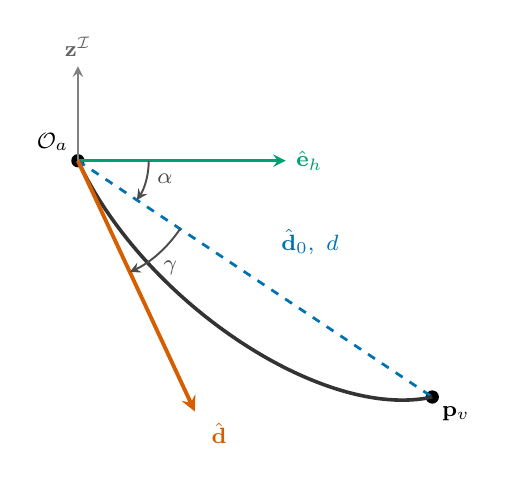
\begin{tikzpicture}[
        >=stealth,
        scale=1.2,
        every node/.style={font=\small},
        chordLine/.style={dashed, okiBlue, line width=1.0pt},
        horizLine/.style={->, okiGreen, line width=1.0pt},
        tetherCurve/.style={black!80, line width=1.3pt},
        tangentVec/.style={->, okiVermillion, line width=1.4pt},
        angleArc/.style={->, line width=0.7pt, black!70}
    ]
        \coordinate (Oa) at (0,0);
        \fill[black] (Oa) circle (2.0pt);
        \node[above left, font=\footnotesize] at (Oa) {$\mathcal{O}_a$};

        \coordinate (Pv) at (3.75,-2.5);
        \fill[black] (Pv) circle (2.0pt);
        \node[below right, font=\footnotesize] at (Pv) {$\mathbf{p}_v$};

        % Local horizontal e_h, within the catenary plane, orthogonal to z^I
        \draw[horizLine] (Oa) -- (2.2,0) node[right, okiGreen, font=\footnotesize] {$\hat{\mathbf{e}}_h$};

        % Chord: taut direction d_0, dashed
        \draw[chordLine] (Oa) -- (Pv);
        \node[above right, okiBlue, font=\footnotesize] at (2.05, -1.1) {$\hat{\mathbf{d}}_0,\ d$};

        % Depression angle alpha, between e_h and the chord
        \draw[angleArc] (Oa) ++(0:0.75) arc (0:-33.69:0.75);
        \node[font=\footnotesize, black!70] at (0.92,-0.19) {$\alpha$};

        % Actual catenary curve
        \draw[tetherCurve] (Oa) .. controls (0.701,-1.503) and (2.604,-2.755) .. (Pv);

        % Tangent (actual tension) direction at O_a
        \draw[tangentVec] (Oa) -- (1.238,-2.654)
            node[below right, okiVermillion, font=\footnotesize, xshift=2pt] {$\hat{\mathbf{d}}$};

        % Angle gamma between the chord and the tangent, drawn further out
        \draw[angleArc] (Oa) ++(-33.69:1.3) arc (-33.69:-65:1.3);
        \node[font=\footnotesize, black!70] at (0.977,-1.139) {$\gamma$};

        % Vertical reference at O_a, i.e. z^I, added back since alpha and gamma
        % are now explicitly measured towards it
        \draw[->, black!50, line width=0.7pt] (Oa) -- (0,1.0) node[above, black!60, font=\footnotesize] {$\mathbf{z}^{\mathcal{I}}$};

    \end{tikzpicture}
    \caption{Tether catenary plane.}
    \label{fig:uav_tether_plane}
\end{figure}


The tension direction at $\mathcal{O}_a$ then follows by tilting $\hat{\mathbf{d}}_0$ further towards the vertical by the angle $\gamma$, within the same plane,
\begin{equation}
    \hat{\mathbf{d}} = \cos(\alpha+\gamma)\,\hat{\mathbf{e}}_h - \sin(\alpha+\gamma)\,\mathbf{z}^{\mathcal{I}},
    \label{eq:uav_tether_direction}
\end{equation}
and the resulting tether force, applied at $\mathcal{O}_a$ and expressed in $\{\mathcal{I}\}$, is
\begin{equation}
    \mathbf{F}_{\mathrm{tether}}^{\mathcal{I}} = T_{\mathrm{tether}}(d)\,\hat{\mathbf{d}} = c_d(\varepsilon_0)\,d\,\hat{\mathbf{d}},
    \label{eq:uav_tether_force}
\end{equation}
with $d$ evaluated at each instant from \eqref{eq:uav_tether_geometry}. Equation~\eqref{eq:uav_tether_force} is the term $\mathbf{F}_{\mathrm{tether}}^{\mathcal{I}}$ introduced in \eqref{eq:uav_newton}.

%%%%%%%%%%%%%%%%%%%%%%%%%%%%%%%%%%%%%%%%%%%%%%%%%%%%%%%%%%%%%%%%%%%%%%%%
%                                                                      %
%     File: Methodology/02_SystemControl.tex                           %
%     Tex Master: ../Thesis.tex                                        %
%                                                                      %
%%%%%%%%%%%%%%%%%%%%%%%%%%%%%%%%%%%%%%%%%%%%%%%%%%%%%%%%%%%%%%%%%%%%%%%%

\section{System Control}
\label{sec:system_control}
\label{chapter:control}

Having established, in Chapter~\ref{chapter:modeling}, the kinematic and dynamic models governing the USV and UAV, the natural next step is to determine how these models can be exploited to compute the control inputs that drive each vehicle along a desired trajectory. Because the two vehicles are physically coupled through the tether, their motion cannot be planned independently without accounting for this interaction, motivating a cooperative control strategy.

The overall control approach is therefore established first, followed by the design of the controllers for each vehicle.

\subsection{Cooperative Control Design}
\label{sec:ctrl_architecture}
Before formulating either controller, the strategies available are weighed against the system's dynamics and its objectives, so that the method chosen suits both vehicles.

\subsubsection{Control Method}
\label{sec:ctrl_method}

Keeping the tether within safe operating conditions depends on how the distance between the two vehicles evolves over time. A controller that only reacts to the current state can correct a violation only after it happens. Anticipating where the system is headed allows corrective action before reaching the safety limits.

A predictive controller does this by repeatedly solving, at each control instant, an optimization problem over a finite look-ahead window. Because the optimization runs over the predicted trajectory rather than the current state alone, requirements such as keeping the tether within safe conditions can be stated as explicit constraints in the problem itself, enforcing them explicitly over the prediction horizon.

The predictions rely on the model of the system dynamics, so their accuracy is tied to how well that model represents the real behaviour. The USV and UAV models derived in Chapter~\ref{chapter:modeling} include nonlinear terms. The predictive controller uses these nonlinear models directly, making non-linear model predictive control the method used for both vehicles.


\subsubsection{Cooperative Architecture}
\label{sec:ctrl_coop_architecture}

The USV and the UAV operate on different timescales. The \gls{usv} moves in the horizontal plane with slow, inertia-dominated motion. The \gls{uav}'s dynamics evolve much faster and demand a finer sampling time. A single \gls{nmpc} built around the combined state of both vehicles would force one prediction horizon and one sampling time onto both, compromising one vehicle's timescale to accommodate the other.

Combining both vehicles into one \gls{nmpc} would also enlarge the state, input, and constraint sets a single solver must handle, making a problem that already runs under real-time constraints harder to solve within the available computation time. Keeping the two problems separate matches each optimization's size to its own vehicle and keeps the computation more manageable in real time.

Each vehicle is therefore controlled by its own \gls{nmpc}. This separation isolates the two controllers from each other's failures: if one solver fails to find a feasible solution, the other vehicle's \gls{nmpc} continues operating on its own well-posed problem.

The tether's safety limits depend on the relative position between the USV and the UAV, so each vehicle's \gls{nmpc} accounts for the other vehicle's position. At every control instant, each controller receives the other vehicle's most recently computed predicted trajectory, and uses it to compute the predicted inter-vehicle distance at the nodes of its own horizon covered by that trajectory. Because the two controllers operate at different sampling intervals, the received predicted trajectory is temporally interpolated and resampled at the receiver's own prediction nodes.

Without this exchange, a vehicle would have to treat the other as stationary or extrapolate its motion from the last known state. Either assumption misrepresents the tether coupling and can drive the system into a constraint violation.

Because the \gls{uav} operates with a finer sampling time and a possibly shorter prediction horizon than the \gls{usv}, its predicted trajectory may cover only part of the \gls{usv}'s horizon. The \gls{usv} therefore enforces the tether constraint only at the nodes covered by the received trajectory, and leaves it inactive at the remaining ones, where no information about the \gls{uav} is available. This avoids constraining the \gls{usv} with an assumed \gls{uav} position that has no basis in the prediction. Since the problem is solved again at every instant, the covered window slides forward with time, and any potential violation is accounted for as soon as it enters it. In the opposite direction no such restriction is needed, since the \gls{usv}'s horizon fully covers that of the \gls{uav}.

Figure~\ref{fig:ctrl_architecture} shows this architecture, with two independent \gls{nmpc} loops, each driving its own vehicle, exchanging predicted horizons to enforce the tether constraint.

\begin{figure}[H]
    \centering
    \definecolor{okiBlue}{rgb}{0.0,0.447,0.698}
    \definecolor{okiGreen}{rgb}{0.0,0.620,0.451}
    \definecolor{okiVermillion}{rgb}{0.835,0.369,0.0}

    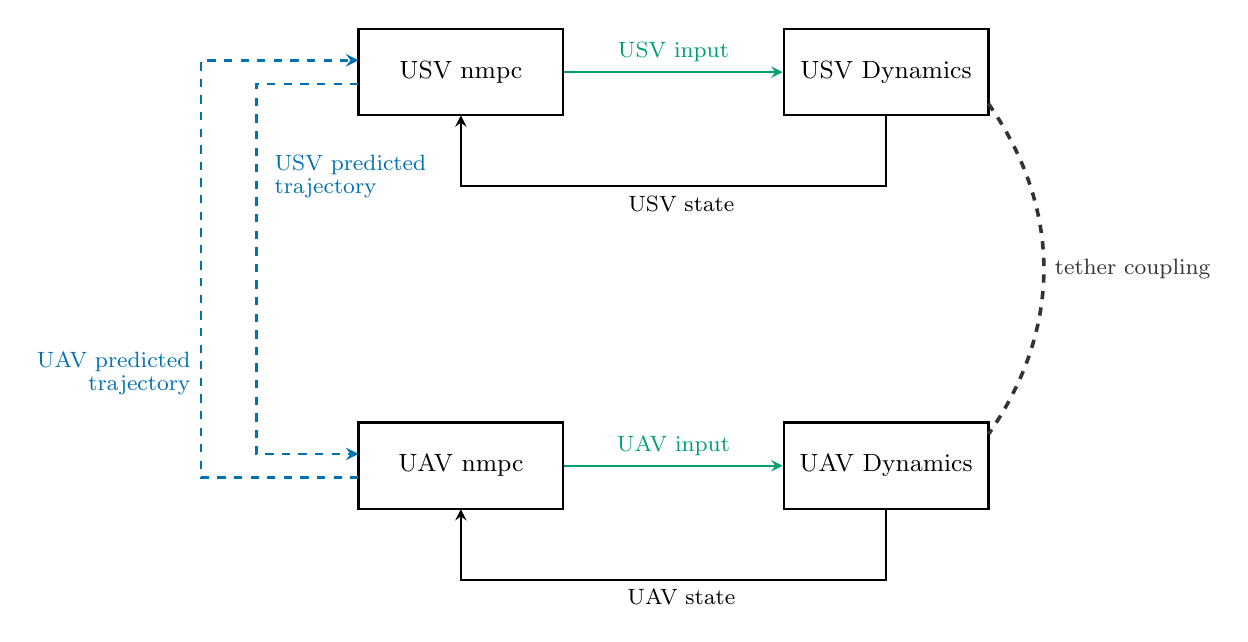
\begin{tikzpicture}[
        >=stealth,
        every node/.style={font=\small},
        boxStyle/.style={draw, rectangle, minimum height=1.1cm, minimum width=2.6cm, align=center, thick},
        sigArrow/.style={->, black, thick},
        exArrow/.style={->, okiBlue, dashed, line width=1.0pt},
        tetherStyle/.style={black!80, dashed, line width=1.3pt}
    ]

        % ---------- USV loop (top) ----------
        \node[boxStyle] (usvnmpc) at (0,5) {USV \gls{nmpc}};
        \node[boxStyle] (usvplant) at (5.4,5) {USV Dynamics};

        \draw[->, okiGreen, thick] (usvnmpc) -- (usvplant)
            node[midway, above, font=\footnotesize] {USV input};

        \draw[sigArrow] (5.4,4.45) -- (5.4,3.55) -- (0,3.55) -- (0,4.45);
        \node[below, font=\footnotesize] at (2.8,3.55) {USV state};

        % ---------- UAV loop (bottom) ----------
        \node[boxStyle] (uavnmpc) at (0,0) {UAV \gls{nmpc}};
        \node[boxStyle] (uavplant) at (5.4,0) {UAV Dynamics};

        \draw[->, okiGreen, thick] (uavnmpc) -- (uavplant)
            node[midway, above, font=\footnotesize] {UAV input};

        \draw[sigArrow] (5.4,-0.55) -- (5.4,-1.45) -- (0,-1.45) -- (0,-0.55);
        \node[below, font=\footnotesize] at (2.8,-1.45) {UAV state};

        % ---------- Coordination exchange between the two NMPCs ----------
        \draw[exArrow] (-1.3,4.85) -- (-2.6,4.85) -- (-2.6,0.15)
            node[pos=0.25, right, align=left, font=\footnotesize, xshift=0.1cm]
            {USV predicted\\[-1pt] trajectory}
            -- (-1.3,0.15);

        \draw[exArrow] (-1.3,-0.15) -- (-3.3,-0.15) -- (-3.3,5.15)
            node[pos=0.25, left, align=right, font=\footnotesize]
            {UAV predicted\\[-1pt] trajectory}
            -- (-1.3,5.15);

        % ---------- Physical tether coupling between plants ----------
        \draw[tetherStyle] (6.7,4.6) to[bend left=35]
            node[midway, right, font=\footnotesize] {tether coupling} (6.7,0.4);

    \end{tikzpicture}
    \caption{Cooperative control architecture diagram.}
    \label{fig:ctrl_architecture}
\end{figure}

\subsection{Nonlinear Model Predictive Control}
\label{sec:ctrl_nmpc_principles}

The vehicle models of Chapter~\ref{chapter:modeling} are continuous-time systems of the form
\begin{equation}
    \dot{\mathbf{x}} = \mathbf{f}\left( \mathbf{x}, \mathbf{u} \right),
    \label{eq:nmpc_dynamics_continuous}
\end{equation}
where $\mathbf{x} \in \mathbb{R}^{n_x}$ is the state vector and $\mathbf{u} \in \mathbb{R}^{n_u}$ is the control input vector.

However, the controller acts at discrete sampling instants $t_k = k T_s$, with the input held constant over each interval $[t_k, t_{k+1})$. Under this assumption, the state at the next instant follows from integrating the dynamics over one sampling interval,
\begin{equation}
    \mathbf{x}(t_{k+1}) = \mathbf{x}(t_k) + \int_{t_k}^{t_{k+1}} \mathbf{f}\left( \mathbf{x}(\tau), \mathbf{u}_k \right) d\tau.
    \label{eq:nmpc_dynamics_integral}
\end{equation}
Since this integral generally has no closed-form solution for nonlinear dynamics, it is approximated by applying a numerical integration scheme to $\mathbf{f}$ over one sampling interval. This defines a one-step discrete map $\boldsymbol\Phi$,
\begin{equation}
    \mathbf{x}_{k+1} = \boldsymbol\Phi\left( \mathbf{x}_k, \mathbf{u}_k \right),
    \label{eq:nmpc_dynamics_general}
\end{equation}
where $\mathbf{x}_k \approx \mathbf{x}(t_k)$ is the system state at instant $k$, so that $\boldsymbol\Phi$ returns the approximate state one sampling interval ahead, given the current state and input.

At every instant $k$, \gls{nmpc} uses this map to predict the future behaviour of the system over a finite look-ahead window of $N$ steps, and computes the input that steers it toward a reference. Denote by $\hat{\mathbf{x}}_{k+i|k}$ and $\hat{\mathbf{u}}_{k+i|k}$ the state and input predicted $i$ steps ahead at instant $k$, for $i = 0, \dots, N$ and $i = 0, \dots, N-1$, respectively. The predicted trajectory starts from the estimated current state,
\begin{equation}
    \hat{\mathbf{x}}_{k|k} = \mathbf{x}_k,
    \label{eq:nmpc_x0}
\end{equation}
and evolves according to the system model,
\begin{equation}
    \hat{\mathbf{x}}_{k+i+1|k} = \boldsymbol\Phi\left( \hat{\mathbf{x}}_{k+i|k}, \hat{\mathbf{u}}_{k+i|k} \right), \quad i = 0, \dots, N-1.
    \label{eq:nmpc_prediction}
\end{equation}

Each predicted step is then scored against a reference trajectory. A stage cost $\ell(\hat{\mathbf{x}}_{k+i|k}, \hat{\mathbf{u}}_{k+i|k})$, typically quadratic, penalizes the tracking error and the control effort at every step of the horizon, and a terminal cost $\ell_f(\hat{\mathbf{x}}_{k+N|k})$ penalizes the tracking error at its final step. Summing both over the horizon gives the total predicted cost,
\begin{equation}
    J = \sum_{i=0}^{N-1} \ell\left( \hat{\mathbf{x}}_{k+i|k}, \hat{\mathbf{u}}_{k+i|k} \right) + \ell_f\left( \hat{\mathbf{x}}_{k+N|k} \right).
    \label{eq:nmpc_cost}
\end{equation}

Minimizing $J$ alone ignores the physical limits of the system, so the prediction is also constrained. The predicted states and inputs must remain within the admissible sets $\mathcal{X}$ and $\mathcal{U}$ at every step of the horizon,
\begin{align}
    \hat{\mathbf{x}}_{k+i|k} &\in \mathcal{X}, \quad i = 0, \dots, N, \label{eq:nmpc_bounds_x} \\
    \hat{\mathbf{u}}_{k+i|k} &\in \mathcal{U}, \quad i = 0, \dots, N-1, \label{eq:nmpc_bounds_u}
\end{align}
where $\mathcal{X}$ and $\mathcal{U}$ collect the admissible states and inputs. These sets may be defined by simple bounds or by general nonlinear inequality constraints of the form $h(\hat{\mathbf{x}}_{k+i|k}, \hat{\mathbf{u}}_{k+i|k}) \le 0$.

Enforcing these sets as hard constraints can make the problem infeasible. If a disturbance pushes the true state outside the admissible set, no predicted trajectory satisfies the constraints, and the solver has no solution to return even though one is required at every sampling instant. To avoid this, a constraint $h(\hat{\mathbf{x}}_{k+i|k}, \hat{\mathbf{u}}_{k+i|k}) \le 0$ can be softened by a slack variable $\sigma \ge 0$,
\begin{equation}
    h(\hat{\mathbf{x}}_{k+i|k}, \hat{\mathbf{u}}_{k+i|k}) \le \sigma,
    \label{eq:nmpc_soft_constraint}
\end{equation}
which allows the constraint to be violated by an amount $\sigma$. The slack becomes an additional decision variable at each step where the constraint is softened, and a penalty
\begin{equation}
    \rho(\sigma) = \mu_{1}\sigma + \mu_{2}\sigma^2, \qquad \mu_{1}, \mu_{2} \ge 0,
    \label{eq:nmpc_slack_penalty}
\end{equation}
is added to the cost $J$ for each slack. Since $\rho(0) = 0$, the solver prefers $\sigma = 0$ whenever the original constraint can be met, and large weights $\mu_1, \mu_2$ keep any violation close to zero.

Assembling the cost, the prediction model, and the constraints defines the optimal control problem solved at every sampling instant $k$,
\begin{align}
    \min_{\hat{\mathbf{x}}_{k+i|k}, \, \hat{\mathbf{u}}_{k+i|k}, \, \hat{\sigma}_{k+i|k}} \quad & J + \sum_{i=0}^{N-1} \rho\left( \hat{\sigma}_{k+i|k} \right) \label{eq:nmpc_ocp_cost} \\
    \text{s.t.} \quad & \hat{\mathbf{x}}_{k|k} = \mathbf{x}_k, \notag \\
    & \hat{\mathbf{x}}_{k+i+1|k} = \boldsymbol\Phi\left( \hat{\mathbf{x}}_{k+i|k}, \hat{\mathbf{u}}_{k+i|k} \right), \quad i = 0, \dots, N-1, \notag \\
    & \hat{\mathbf{x}}_{k+i|k} \in \mathcal{X}, \quad i = 0, \dots, N, \notag \\
    & \hat{\mathbf{u}}_{k+i|k} \in \mathcal{U}, \quad i = 0, \dots, N-1, \notag \\
    & h\left( \hat{\mathbf{x}}_{k+i|k}, \hat{\mathbf{u}}_{k+i|k} \right) \le \hat{\sigma}_{k+i|k}, \quad \hat{\sigma}_{k+i|k} \ge 0, \quad i = 0, \dots, N-1. \notag
\end{align}

Solving this problem returns a full predicted input sequence, $\hat{\mathbf{u}}_{k|k}, \dots, \hat{\mathbf{u}}_{k+N-1|k}$, but only its first element, $\hat{\mathbf{u}}_{k|k}$, is applied to the system. At the next instant, $k+1$, the state is estimated again and the problem is solved again from $\hat{\mathbf{x}}_{k+1|k+1} = \mathbf{x}_{k+1}$, with the horizon shifted one step forward. This strategy, known as the receding horizon principle, computes every input from the latest state estimate, so the controller can correct for disturbances and model errors that the previous prediction did not anticipate.


\subsection{USV NMPC}
\label{sec:ctrl_usv_mpc}

The USV NMPC computes, at every sampling instant, the thruster commands that best track a reference trajectory over a finite prediction horizon, subject to the vessel's dynamics, the physical limits of its actuators, and the tether workspace. It predicts the vessel's motion with the model derived in Chapter~\ref{chapter:modeling}, and solves a constrained optimization problem at each step to obtain the commands applied to the thrusters.

\subsubsection*{Predictive Model}

The vessel model of Chapter~\ref{chapter:modeling} is driven by the resultant thrust force and moment $\boldsymbol\tau = [X,Y,N]^\top$, which are obtained from the physical actuator commands $T_L, T_R, \alpha_L, \alpha_R$ through the allocation
\begin{equation}
    X = T_L\cos\alpha_L + T_R\cos\alpha_R, \qquad Y = T_L\sin\alpha_L + T_R\sin\alpha_R,
    \label{eq:usv_mpc_alloc_force}
\end{equation}
\begin{equation}
    N = -x_{arm}\big(T_L\sin\alpha_L+T_R\sin\alpha_R\big) - y_{arm}\big(T_L\cos\alpha_L-T_R\cos\alpha_R\big).
    \label{eq:usv_mpc_alloc_moment}
\end{equation}

Since the controller ultimately has to command $T_L, T_R, \alpha_L, \alpha_R$, the \gls{nmpc} is formulated directly in terms of these variables, rather than choosing $\boldsymbol\tau$ and allocating it separately. This way, the limits of the physical actuators can be imposed directly in the optimization problem.

Each thruster is limited both in the thrust and azimuth it can deliver,
\begin{equation}
    T_{L,min} \le T_L \le T_{L,max}, \quad T_{R,min} \le T_R \le T_{R,max}, \quad \alpha_{L,min} \le \alpha_L \le \alpha_{L,max}, \quad \alpha_{R,min} \le \alpha_R \le \alpha_{R,max},
    \label{eq:usv_mpc_state_bounds}
\end{equation}
and in how fast it can change them,
\begin{equation}
    |\dot{T}_L| \le \dot{T}_{L,max}, \quad |\dot{T}_R| \le \dot{T}_{R,max}, \quad |\dot{\alpha}_L| \le \dot{\alpha}_{L,max}, \quad |\dot{\alpha}_R| \le \dot{\alpha}_{R,max}.
    \label{eq:usv_mpc_input_bounds}
\end{equation}
The rate limits act on the time derivatives of the commands, so imposing them directly as bounds requires these derivatives to become the control input,
\begin{equation}
    \mathbf{u}_v = [\dot{T}_L, \dot{T}_R, \dot{\alpha}_L, \dot{\alpha}_R]^\top \in \mathbb{R}^4,
    \label{eq:usv_mpc_input_augmented}
\end{equation}
which in turn makes $T_L, T_R, \alpha_L, \alpha_R$ part of the state vector,
\begin{equation}
    \mathbf{x}_v = [x, y, \psi, u, v, r,\ T_L, T_R, \alpha_L, \alpha_R]^\top \in \mathbb{R}^{10}.
    \label{eq:usv_mpc_state_augmented}
\end{equation}
With this choice, the range limits act on the state, and the rate limits act directly on the input.

With $\mathbf{x}_v$ and $\mathbf{u}_v$ defined, the prediction model $\dot{\mathbf{x}}_v = \mathbf{f}_v(\mathbf{x}_v,\mathbf{u}_v)$ is assembled from the vessel kinematics and dynamics.

The kinematics are given by \eqref{eq:usv_kinematics_planar} and \eqref{eq:usv_psi_dot},
\begin{equation}
    \dot x = u\cos\psi - v\sin\psi, \qquad \dot y = u\sin\psi + v\cos\psi, \qquad \dot\psi = r.
    \label{eq:usv_mpc_kinematics}
\end{equation}

The dynamics follow \eqref{eq:usv_udot}--\eqref{eq:usv_rdot}, with $X,Y,N$ given by \eqref{eq:usv_mpc_alloc_force}--\eqref{eq:usv_mpc_alloc_moment} in terms of the thruster state,
\begin{equation}
    \dot u = \frac{1}{m}\Big[X - \big(X_u+X_{uu}^{\pm}|u|\big)u\Big] + vr,
    \label{eq:usv_mpc_udot}
\end{equation}
\begin{equation}
    \dot v = \frac{1}{m}\Big[Y - \big(Y_v+Y_{vv}|v|\big)v\Big] - ur,
    \label{eq:usv_mpc_vdot}
\end{equation}
\begin{equation}
    \dot r = \frac{1}{I_z}\Big[N - \big(N_r+N_{rr}|r|\big)r\Big].
    \label{eq:usv_mpc_rdot}
\end{equation}

Finally, $\dot T_L,\dot T_R,\dot\alpha_L,\dot\alpha_R$ appear directly as the components of $\mathbf{u}_v$,
\begin{equation}
    \dot T_L = \dot T_L, \qquad \dot T_R = \dot T_R, \qquad \dot\alpha_L = \dot\alpha_L, \qquad \dot\alpha_R = \dot\alpha_R.
    \label{eq:usv_mpc_thruster_rates}
\end{equation}

Discretization over a sampling interval $T_s$, following Section~\ref{sec:ctrl_nmpc_principles}, gives the one-step map $\boldsymbol\Phi_v$ such that $\hat{\mathbf{x}}_{v,k+i+1|k} = \boldsymbol\Phi_v\big(\hat{\mathbf{x}}_{v,k+i|k}, \hat{\mathbf{u}}_{v,k+i|k}\big)$ approximates the solution of $\dot{\mathbf{x}}_v = \mathbf{f}_v(\mathbf{x}_v,\mathbf{u}_v)$ over one sampling interval.


\subsubsection*{Cost and Constraints}
 
Let $\mathbf{p} = [x,y]^\top$ denote the position, $\psi$ the heading, and $\boldsymbol{\nu} = [u,v,r]^\top$ the body-fixed velocities, with $\mathbf{p}_{ref}$, $\psi_{ref}$, and $\boldsymbol{\nu}_{ref}$ the corresponding references from a given trajectory.

Tracking the reference position is penalized quadratically as
\begin{equation}
    \|\mathbf{p}-\mathbf{p}_{ref}\|^2_{Q_p},
    \label{eq:usv_mpc_cost_pos}
\end{equation}
where $\|\boldsymbol\xi\|^2_W \coloneqq \boldsymbol\xi^\top W \boldsymbol\xi$ for a positive semi-definite weighting matrix $W$, which sets the relative importance of each component of $\boldsymbol\xi$ in the cost.

Tracking the heading reference is penalized as
\begin{equation}
    q_\psi\big(1-\cos(\psi-\psi_{ref})\big),
    \label{eq:usv_mpc_cost_heading}
\end{equation}
where $q_\psi \ge 0$ is a scalar weight setting the relative importance of heading tracking.

Both $\psi$ and $\psi_{ref}$ are angles represented within an interval of width $2\pi$, such as $(-\pi,\pi]$. When they lie near opposite ends of this interval, their raw difference $\psi-\psi_{ref}$ approaches $\pm2\pi$, even though the two headings are then almost identical. As $\cos(\cdot)$ has period $2\pi$, its value approaches one whenever $\psi-\psi_{ref}$ is near zero or $\pm2\pi$, so the cost \eqref{eq:usv_mpc_cost_heading} is near zero in both cases, correctly reflecting that the two headings are almost identical.

Tracking the reference velocity is penalized in the same way as the position,
\begin{equation}
    \|\boldsymbol{\nu}-\boldsymbol{\nu}_{ref}\|^2_{Q_\nu}.
    \label{eq:usv_mpc_cost_vel}
\end{equation}

The thruster commands $T_L, T_R, \alpha_L, \alpha_R$ are regularized directly as
\begin{equation}
    \big\|[T_L,T_R,\alpha_L,\alpha_R]^\top\big\|^2_{Q_\tau},
    \label{eq:usv_mpc_cost_reg}
\end{equation}
discouraging thrust and azimuth commands larger than necessary to track the reference.

The last term penalizes $\mathbf{u}_v$, the rate of change of the thruster commands,
\begin{equation}
    \big\|[\dot{T}_L, \dot{T}_R, \dot{\alpha}_L, \dot{\alpha}_R]^\top\big\|^2_{R},
    \label{eq:usv_mpc_cost_rate}
\end{equation}
discouraging abrupt changes in thrust and azimuth between consecutive instants.

Summing \eqref{eq:usv_mpc_cost_pos}--\eqref{eq:usv_mpc_cost_rate} gives the stage cost
\begin{equation}
    \begin{aligned}
        \ell(\mathbf{x}_v, \mathbf{u}_v) = {} & \|\mathbf{p}-\mathbf{p}_{ref}\|^2_{Q_p} + q_\psi\big(1-\cos(\psi-\psi_{ref})\big) + \|\boldsymbol{\nu}-\boldsymbol{\nu}_{ref}\|^2_{Q_\nu} \\
        & + \big\|[T_L,T_R,\alpha_L,\alpha_R]^\top\big\|^2_{Q_\tau} + \big\|[\dot{T}_L, \dot{T}_R, \dot{\alpha}_L, \dot{\alpha}_R]^\top\big\|^2_{R}.
    \end{aligned}
    \label{eq:usv_mpc_stage_cost}
\end{equation}

The terminal cost $\ell_f$ penalizes the last predicted state, so that the optimizer does not disregard where the vessel ends up at the end of the horizon. It equals the stage cost \eqref{eq:usv_mpc_stage_cost} without the input rate term, since no control input is chosen at the final node:
\begin{equation}
    \ell_f(\mathbf{x}_v) = \|\mathbf{p}-\mathbf{p}_{ref}\|^2_{Q_p} + q_\psi\big(1-\cos(\psi-\psi_{ref})\big) + \|\boldsymbol{\nu}-\boldsymbol{\nu}_{ref}\|^2_{Q_\nu} + \big\|[T_L,T_R,\alpha_L,\alpha_R]^\top\big\|^2_{Q_\tau}.
    \label{eq:usv_mpc_terminal_cost}
\end{equation}
 
The thruster limits introduced in the predictive model enter the optimization problem as constraints. Since thrust and azimuth are components of the state, their range limits define the admissible state set
\begin{equation}
    \mathcal{X} = \left\{ \mathbf{x}_v : \;
    \begin{aligned}
        & T_{L,min} \le T_L \le T_{L,max}, \quad T_{R,min} \le T_R \le T_{R,max}, \\
        & \alpha_{L,min} \le \alpha_L \le \alpha_{L,max}, \quad \alpha_{R,min} \le \alpha_R \le \alpha_{R,max}
    \end{aligned}
    \right\},
    \label{eq:usv_mpc_set_X}
\end{equation}
while the limits on their rates of change, which act on the input, define the admissible input set
\begin{equation}
    \mathcal{U} = \left\{ \mathbf{u}_v : \;
    \begin{aligned}
        & |\dot{T}_L| \le \dot{T}_{L,max}, \quad |\dot{T}_R| \le \dot{T}_{R,max}, \\
        & |\dot{\alpha}_L| \le \dot{\alpha}_{L,max}, \quad |\dot{\alpha}_R| \le \dot{\alpha}_{R,max}
    \end{aligned}
    \right\}.
    \label{eq:usv_mpc_set_U}
\end{equation}

The last constraint couples the vessel to the UAV through the tether, and is the only one that depends on the other vehicle. The tether limits the distance between its attachment point on the vessel deck and the UAV to a maximum admissible separation $d_{max}$. The attachment point is vertically aligned with the origin of the vessel's body frame, at a fixed height $z_t$ in the inertial frame, so its position is $(x, y, z_t)$. Along the horizon, the USV controller uses the UAV's most recently computed predicted trajectory $\hat{\mathbf{p}}_a = [\hat x_a, \hat y_a, \hat z_a]^\top$, temporally resampled at the vessel's prediction nodes covered by it, to compute the squared distance between the attachment point and the UAV,
\begin{equation}
    d^2 = (x - \hat x_a)^2 + (y - \hat y_a)^2 + (\hat z_a - z_t)^2.
    \label{eq:usv_mpc_tether_distance}
\end{equation}
The requirement $d^2 \le d_{max}^2$ is enforced as a soft constraint through a slack variable $\sigma \ge 0$,
\begin{equation}
    \underbrace{d^2 - d_{max}^2}_{h(\mathbf{x}_v)} \le \sigma,
    \label{eq:usv_mpc_tether_constraint}
\end{equation}
which is penalized by $\rho(\sigma)$ as in \eqref{eq:nmpc_slack_penalty}, with large weights $\mu_1$ and $\mu_2$ so that violations remain small whenever geometrically feasible.

\subsubsection*{Optimal Control Problem}
 
At every sampling instant $k$, the kinematic and dynamic components of the initial state come from the vessel's current estimate, while the thruster components use the last command actually applied:
\begin{equation}
    \mathbf{x}_{v,k} = \big[x_k, y_k, \psi_k, u_k, v_k, r_k,\ T_{L,k-1}, T_{R,k-1}, \alpha_{L,k-1}, \alpha_{R,k-1}\big]^\top.
    \label{eq:usv_mpc_initial_condition}
\end{equation}
Starting from the last applied command ensures that the rate limits in \eqref{eq:usv_mpc_input_bounds} are enforced relative to the actual thruster values, so the first input chosen is always attainable by the thrusters.

The references and the \gls{uav}'s predicted trajectory are given data at each instant. Since the \gls{uav}'s predicted trajectory can be shorter than the vessel's horizon, let $N_c \le N$ denote the last node of the vessel's horizon covered by it. The tether constraint, and its slack, are enforced only for $i = 0, \dots, N_c$.
 
Assembling the cost, the model, and the constraints gives the optimal control problem the USV solves at every sampling instant:
\begin{align}
    \min_{\hat{\mathbf{x}}_v,\, \hat{\mathbf{u}}_v,\, \hat{\sigma}} \quad & \sum_{i=0}^{N-1} \ell\big(\hat{\mathbf{x}}_{v,k+i|k}, \hat{\mathbf{u}}_{v,k+i|k}\big) + \ell_f\big(\hat{\mathbf{x}}_{v,k+N|k}\big) + \sum_{i=0}^{N_c} \rho\big(\hat\sigma_{k+i|k}\big) \notag \\
    \text{s.t.} \quad & \hat{\mathbf{x}}_{v,k|k} = \mathbf{x}_{v,k}, \notag \\
    & \hat{\mathbf{x}}_{v,k+i+1|k} = \boldsymbol\Phi_v\big(\hat{\mathbf{x}}_{v,k+i|k}, \hat{\mathbf{u}}_{v,k+i|k}\big), \quad i = 0, \dots, N-1, \notag \\
    & \hat{\mathbf{x}}_{v,k+i|k} \in \mathcal{X}, \quad i = 0, \dots, N, \notag \\
    & \hat{\mathbf{u}}_{v,k+i|k} \in \mathcal{U}, \quad i = 0, \dots, N-1, \notag \\
    & h\big(\hat{\mathbf{x}}_{v,k+i|k}\big) \le \hat\sigma_{k+i|k}, \quad \hat\sigma_{k+i|k} \ge 0, \quad i = 0, \dots, N_c. \label{eq:usv_mpc_ocp}
\end{align}
The vessel's low-level actuators receive the integrated thruster commands $T_{L,k}, T_{R,k}, \alpha_{L,k}, \alpha_{R,k}$, obtained by integrating the first optimal input rate $\hat{\mathbf{u}}_{v,k|k}$ over the sampling interval $T_s$. These become the thruster components of the initial state at the subsequent sampling instant.
 
%%%%%%%%%%%%%%%%%%%%%%%%%%%%%%%%%%%%%%%%%%%%%%%%%%%%%%%%%%%%%%%%%%%%%%%%%%%%%%%%%%%%%%%%%
\subsection{UAV NMPC}
\label{sec:ctrl_uav_mpc}

The UAV NMPC computes, at every sampling instant, the thrust and attitude commands that best track a reference trajectory over a finite prediction horizon, subject to the vehicle's dynamics, its actuation limits, and the tether workspace. It predicts the vehicle's motion with the model derived in Chapter~\ref{chapter:modeling}, and solves a constrained optimization problem at each step to obtain the commands applied to the vehicle.

\subsubsection*{Predictive Model}

The input $\mathbf{u}_a = [T,\phi,\theta,\psi]^\top$ of the vehicle model defined in Chapter~\ref{chapter:modeling} commands the thrust and the attitude directly, assuming each of them is reached instantaneously.

Similarly to the thrusters of the USV, the attitude of the \gls{uav} cannot change arbitrarily fast, and its rate of change is limited,
\begin{equation}
    |\dot\phi| \le \dot\phi_{max}, \quad |\dot\theta| \le \dot\theta_{max}, \quad |\dot\psi| \le \dot\psi_{max}.
    \label{eq:uav_mpc_rate_bounds}
\end{equation}
Since these limits act on the time derivatives of the attitude, imposing them directly as bounds requires the rates to be part of the control input,
\begin{equation}
    \mathbf{u}_a = [\dot\phi,\dot\theta,\dot\psi,T]^\top \in \mathbb{R}^4,
    \label{eq:uav_mpc_input_augmented}
\end{equation}
which makes $\phi,\theta,\psi$ part of the state vector,
\begin{equation}
    \mathbf{x}_a = [x,y,z,\dot x,\dot y,\dot z,\ \phi,\theta,\psi]^\top \in \mathbb{R}^{9}.
    \label{eq:uav_mpc_state_augmented}
\end{equation}

With $\mathbf{x}_a$ and $\mathbf{u}_a$ defined, the prediction model $\dot{\mathbf{x}}_a = \mathbf{f}_a(\mathbf{x}_a,\mathbf{u}_a)$ is assembled from the \gls{uav} kinematics and dynamics, together with the attitude rates.

The kinematics are the trivial identity already used in \eqref{eq:uav_kinematics},
\begin{equation}
    \dot x = \dot x, \qquad \dot y = \dot y, \qquad \dot z = \dot z.
    \label{eq:uav_mpc_kinematics}
\end{equation}

The translational dynamics follow \eqref{eq:uav_dynamics}, with the thrust term expanded and the tether force $\mathbf{F}_{\mathrm{tether}}^{\mathcal{I}} = [F_{\mathrm{tether},x}^{\mathcal{I}}, F_{\mathrm{tether},y}^{\mathcal{I}}, F_{\mathrm{tether},z}^{\mathcal{I}}]^\top$ given by \eqref{eq:uav_tether_geometry}--\eqref{eq:uav_tether_force},
\begin{equation}
    \ddot x = \frac{T}{m}\big(\cos\psi\sin\theta\cos\phi+\sin\psi\sin\phi\big) + \frac{1}{m}F_{\mathrm{tether},x}^{\mathcal{I}},
    \label{eq:uav_mpc_xddot}
\end{equation}
\begin{equation}
    \ddot y = \frac{T}{m}\big(\sin\psi\sin\theta\cos\phi-\cos\psi\sin\phi\big) + \frac{1}{m}F_{\mathrm{tether},y}^{\mathcal{I}},
    \label{eq:uav_mpc_yddot}
\end{equation}
\begin{equation}
    \ddot z = \frac{T}{m}\cos\theta\cos\phi - g + \frac{1}{m}F_{\mathrm{tether},z}^{\mathcal{I}}.
    \label{eq:uav_mpc_zddot}
\end{equation}

Finally, $\dot\phi,\dot\theta,\dot\psi$ appear directly as the first three components of $\mathbf{u}_a$,
\begin{equation}
    \dot\phi = \dot\phi, \qquad \dot\theta = \dot\theta, \qquad \dot\psi = \dot\psi.
    \label{eq:uav_mpc_attitude_rates}
\end{equation}

Discretization over a sampling interval $T_s$, following Section~\ref{sec:ctrl_nmpc_principles}, gives the one-step map $\boldsymbol\Phi_a$ such that $\hat{\mathbf{x}}_{a,k+i+1|k} = \boldsymbol\Phi_a\big(\hat{\mathbf{x}}_{a,k+i|k},\hat{\mathbf{u}}_{a,k+i|k}\big)$ approximates the solution of $\dot{\mathbf{x}}_a = \mathbf{f}_a(\mathbf{x}_a,\mathbf{u}_a)$ over one sampling interval.

\subsubsection*{Cost and Constraints}

Let $\mathbf{p} = [x,y,z]^\top$ and $\mathbf{v} = [\dot x,\dot y,\dot z]^\top$ denote the position and velocity, with $\mathbf{p}_{ref}$ and $\mathbf{v}_{ref}$ the corresponding references.

Tracking the reference position and velocity is penalized quadratically as
\begin{equation}
    \|\mathbf{p}-\mathbf{p}_{ref}\|^2_{Q_p} + \|\mathbf{v}-\mathbf{v}_{ref}\|^2_{Q_v}.
    \label{eq:uav_mpc_cost_track}
\end{equation}

The next term penalizes $\phi,\theta$ directly, rather than comparing them against any reference,
\begin{equation}
    \big\|[\phi,\theta]^\top\big\|^2_{Q_{tilt}},
    \label{eq:uav_mpc_cost_tilt}
\end{equation}
discouraging attitude larger than necessary to track the reference.

The next term penalizes the yaw error, but rather than tracking a fixed yaw angle, $\psi$ is aligned with the direction to a reference point $\mathbf{p}_{b,ref} = [x_{b,ref},y_{b,ref}]^\top$, itself possibly varying along the horizon,
\begin{equation}
    \mathbf{b} = \mathbf{p}_{b,ref} - \mathbf{p}_{xy},
    \label{eq:uav_mpc_yaw_direction}
\end{equation}
where $\mathbf{p}_{xy}=[x,y]^\top$. Since $\psi$ is an angle, the periodicity issue discussed for \eqref{eq:usv_mpc_cost_heading} also applies here, and it is handled by expressing the error as an alignment between $\psi$ and the bearing vector $\mathbf{b}$, rather than as a difference between two angles,
\begin{equation}
    q_\psi\left(1 - \frac{\cos\psi\,b_x + \sin\psi\,b_y}{\sqrt{\|\mathbf{b}\|^2 + \epsilon}}\right),
    \label{eq:uav_mpc_cost_yaw}
\end{equation}
where $q_\psi \ge 0$ is a scalar weight setting the relative importance of yaw tracking, and $\epsilon > 0$ is a small constant that keeps the term well defined when the \gls{uav} is above the reference point, where the bearing is undefined. This term is minimized when $\psi$ points along $\mathbf{b}$.

The last term penalizes the input $\mathbf{u}_a$ relative to a nominal hover reference $\mathbf{u}_{a,ref} = [0,0,0,mg]^\top$, since the thrust cannot be penalized toward zero without opposing gravity,
\begin{equation}
    \|\mathbf{u}_a - \mathbf{u}_{a,ref}\|^2_{R},
    \label{eq:uav_mpc_cost_input}
\end{equation}
so that the attitude rates are regularized toward zero, while the thrust is penalized only for deviating from the hover value.

Summing the tracking, tilt, yaw, and input penalties in \eqref{eq:uav_mpc_cost_track}, \eqref{eq:uav_mpc_cost_tilt}, \eqref{eq:uav_mpc_cost_yaw}, and \eqref{eq:uav_mpc_cost_input} gives the stage cost
\begin{equation}
    \begin{aligned}
        \ell(\mathbf{x}_a,\mathbf{u}_a) = {} & \|\mathbf{p}-\mathbf{p}_{ref}\|^2_{Q_p} + \|\mathbf{v}-\mathbf{v}_{ref}\|^2_{Q_v} + \big\|[\phi,\theta]^\top\big\|^2_{Q_{tilt}} \\
        & + q_\psi\left(1 - \frac{\cos\psi\,b_x + \sin\psi\,b_y}{\|\mathbf{b}\|}\right) + \|\mathbf{u}_a-\mathbf{u}_{a,ref}\|^2_R.
    \end{aligned}
    \label{eq:uav_mpc_stage_cost}
\end{equation}

The terminal cost $\ell_f$ penalizes the last predicted state, so that the optimizer does not disregard where the \gls{uav} ends up at the end of the horizon. It equals the stage cost \eqref{eq:uav_mpc_stage_cost} without the input term, since no input is chosen at the final node:
\begin{equation}
    \begin{aligned}
        \ell_f(\mathbf{x}_a) = {} & \|\mathbf{p}-\mathbf{p}_{ref}\|^2_{Q_p} + \|\mathbf{v}-\mathbf{v}_{ref}\|^2_{Q_v} + \big\|[\phi,\theta]^\top\big\|^2_{Q_{tilt}} \\
        & + q_\psi\left(1 - \frac{\cos\psi\,b_x + \sin\psi\,b_y}{\|\mathbf{b}\|}\right).
    \end{aligned}
    \label{eq:uav_mpc_terminal_cost}
\end{equation}

The vehicle's operating envelope bounds the altitude, translational velocity, and attitude. To guarantee safe clearance above the water surface and vessel deck, the vehicle is restricted to $z \ge z_{min}$. Furthermore, because horizontal and vertical velocities are limited by distinct physical factors, the vehicle's speed and tilt are bounded separately:
\begin{equation}
    z \ge z_{min}, \quad \big\|[\dot x,\dot y]^\top\big\| \le v_{xy,max}, \quad |\dot z| \le v_{z,max}, \quad |\phi| \le \phi_{max}, \quad |\theta| \le \theta_{max}.
    \label{eq:uav_mpc_state_bounds}
\end{equation}
Unlike the thruster commands of the USV, the velocity and attitude are subject to external disturbances such as wind, which can push the true state past these bounds regardless of what the \gls{nmpc} has commanded. The bounds of \eqref{eq:uav_mpc_state_bounds} are therefore softened as in \eqref{eq:nmpc_soft_constraint}, each with its own slack variable $\sigma_j \ge 0$, $j=1,\dots,5$:
\begin{align}
    \underbrace{z_{min} - z}_{h_1(\mathbf{x}_a)} &\le \sigma_1, \label{eq:uav_mpc_slack_z} \\
    \underbrace{\big\|[\dot x,\dot y]^\top\big\| - v_{xy,max}}_{h_2(\mathbf{x}_a)} &\le \sigma_2, \label{eq:uav_mpc_slack_vxy} \\
    \underbrace{|\dot z| - v_{z,max}}_{h_3(\mathbf{x}_a)} &\le \sigma_3, \label{eq:uav_mpc_slack_vz} \\
    \underbrace{|\phi| - \phi_{max}}_{h_4(\mathbf{x}_a)} &\le \sigma_4, \label{eq:uav_mpc_slack_phi} \\
    \underbrace{|\theta| - \theta_{max}}_{h_5(\mathbf{x}_a)} &\le \sigma_5. \label{eq:uav_mpc_slack_theta}
\end{align}
Each slack is penalized by $\rho_j(\sigma_j)$ as in \eqref{eq:nmpc_slack_penalty}, with weights $\mu_{1,j}$ and $\mu_{2,j}$.

The attitude rate limits of the predictive model \eqref{eq:uav_mpc_rate_bounds} and the thrust range are the only hard constraints, and they act on the input, defining the admissible input set
\begin{equation}
    \mathcal{U} = \left\{ \mathbf{u}_a : \;
    \begin{aligned}
        & |\dot\phi| \le \dot\phi_{max}, \quad |\dot\theta| \le \dot\theta_{max}, \quad |\dot\psi| \le \dot\psi_{max}, \\
        & T_{min} \le T \le T_{max}
    \end{aligned}
    \right\}.
    \label{eq:uav_mpc_input_set}
\end{equation}

The last constraint couples the \gls{uav} to the vessel through the tether, and is the only one that depends on the other vehicle. As for the vessel, it limits the distance between the \gls{uav} and the tether attachment point, described in Section~\ref{sec:ctrl_usv_mpc}, to the maximum admissible separation $d_{max}$. The attachment point on the \gls{usv} is located at $(\hat x_v, \hat y_v, z_t)$, where the horizontal position $\hat{\mathbf{p}}_v = [\hat x_v, \hat y_v]^\top$ at each node is taken from the vessel's most recently computed predicted trajectory, temporally resampled at the \gls{uav}'s prediction nodes, and $z_t$ is the height of the attachment point. Since the vessel's horizon covers that of the \gls{uav}, the constraint is enforced at every node. The squared distance between the \gls{uav} and the attachment point is
\begin{equation}
    d^2 = (x-\hat x_v)^2 + (y-\hat y_v)^2 + (z-z_t)^2.
    \label{eq:uav_mpc_tether_distance}
\end{equation}
The requirement $d^2 \le d_{max}^2$ is enforced as a soft constraint through a slack variable $\sigma_6 \ge 0$,
\begin{equation}
    \underbrace{d^2 - d_{max}^2}_{h_6(\mathbf{x}_a)} \le \sigma_6,
    \label{eq:uav_mpc_tether_constraint}
\end{equation}
which is penalized by $\rho_6(\sigma_6)$ as in \eqref{eq:nmpc_slack_penalty}, with large weights $\mu_{1,6}$ and $\mu_{2,6}$ so that violations remain small.

Together, the minimum altitude $z_{min}$ and the maximum tether separation $d_{max}$ delimit the workspace of the \gls{uav}, illustrated in Figure~\ref{fig:uav_operating_region}.

\begin{figure}[H]
    \centering
    % Colors: Okabe-Ito colorblind-safe qualitative palette (Okabe and Ito, 2008)
    \definecolor{okiBlue}{rgb}{0.0,0.447,0.698}
    \definecolor{okiOrange}{rgb}{0.902,0.624,0.0}
    \definecolor{okiVermillion}{rgb}{0.835,0.369,0.0}

    \begin{tikzpicture}[
        >=stealth,
        label/.style={black,font=\small},
        tether/.style={draw,line width=1.5pt,darkgray,smooth}
    ]
        % -- PARAMETERS (drawing units, not to scale) --
        \pgfmathsetmacro{\zt}{0.9}      % attachment height
        \pgfmathsetmacro{\zmin}{2.0}    % minimum UAV altitude
        \pgfmathsetmacro{\dmax}{4.5}    % maximum separation
        \pgfmathsetmacro{\aZ}{asin((\zmin-\zt)/\dmax)}   % circle angle at z = z_min (right)
        \pgfmathsetmacro{\aZL}{180-\aZ}                  % same, left
        \pgfmathsetmacro{\aW}{asin(-\zt/\dmax)}          % circle angle at water surface (right)
        \pgfmathsetmacro{\aWL}{180-\aW}                  % same, left
        \coordinate (C) at (0,\zt);

        % -- OPERATING REGION (circular segment above z_min) --
        \fill[okiBlue!15] ($(C)+(\aZ:\dmax)$) arc[start angle=\aZ, end angle=\aZL, radius=\dmax] -- cycle;
        \node[label,okiBlue!80!black,align=center] at (-1.5,3.6) {UAV operating\\region};

        % -- WATER SURFACE (z = 0) --
        \draw[black, dashed, line width=0.8pt] (-5.6,0) -- (5.6,0) node[right, font=\scriptsize, black!80] {Water Surface ($z^{\mathcal{I}}=0$)};

        % -- MINIMUM ALTITUDE --
        \draw[black!70, dash dot, line width=0.8pt] (-5.2,\zmin) -- (5.2,\zmin);
        \draw[<->, thin] (-3.2,0) -- (-3.2,\zmin) node[midway,left,font=\small] {$z_{min}$};

        % -- MAXIMUM SEPARATION CIRCLE (solid where admissible, dashed below z_min) --
        \draw[okiBlue, line width=1.3pt] ($(C)+(\aZ:\dmax)$) arc[start angle=\aZ, end angle=\aZL, radius=\dmax];
        \draw[okiBlue, dashed, line width=1.1pt] ($(C)+(\aW:\dmax)$) arc[start angle=\aW, end angle=\aZ, radius=\dmax];
        \draw[okiBlue, dashed, line width=1.1pt] ($(C)+(\aZL:\dmax)$) arc[start angle=\aZL, end angle=\aWL, radius=\dmax];
        \draw[okiBlue, line width=0.8pt] (C) -- ++(20:\dmax) node[midway,above,sloped,font=\small] {$d_{max}$};

        % -- USV (catamaran seen from the side) --
        \begin{scope}[shift={(0,0.45)}]
            \draw[thick,fill=gray!30] (-1.2,-0.45) -- (0.8,-0.45) to[out=0,in=-120] (1.3,-0.15) -- (-1.2,-0.15) -- cycle;
            \draw[line width=1.5pt,black] (-0.6,-0.15) -- (-0.3,0.3);
            \draw[line width=1.5pt,black] (0.6,-0.15) -- (0.3,0.3);
            \draw[thick,fill=gray!50] (-0.5,0.3) rectangle (0.5,0.45);
            \coordinate (Pa) at (0,0.45);
            \fill[okiVermillion] (Pa) circle (2.5pt) node[above left,font=\scriptsize,black] {Anchor};
        \end{scope}

        % -- ATTACHMENT HEIGHT z_t, with guide line to the anchor point --
        \draw[<->, thin] (-2.0,0) -- (-2.0,\zt) node[midway,left,font=\small] {$z_t$};
        \draw[black!70, dashed, thin] (-2.0,\zt) -- (Pa);

        % -- UAV (inside the operating region) --
        \coordinate (Oa) at (1.6,3.4);
        \begin{scope}[shift={(Oa)}, rotate=-15]
            \draw[thick,line width=1.5pt,black] (-0.6,-0.15) -- (0.6,0.15);
            \draw[thick,line width=1.5pt,black] (-0.5,0.15) -- (0.5,-0.15);
            \fill[black] (0,0) circle (3.5pt);
            \draw[gray, thin] (-0.6,-0.1) ellipse (3pt and 0.8pt);
            \draw[gray, thin] (0.6,0.2) ellipse (3pt and 0.8pt);
            \draw[gray, thin] (-0.5,0.2) ellipse (3pt and 0.8pt);
            \draw[gray, thin] (0.5,-0.1) ellipse (3pt and 0.8pt);
        \end{scope}

        % -- TETHER --
        \draw[tether] (Pa) .. controls ($(Pa)+(1.0,0.6)$) and ($(Oa)+(-0.3,-1.0)$) .. (Oa);

    \end{tikzpicture}
    \caption{Operating region of the \gls{uav}.}
    \label{fig:uav_operating_region}
\end{figure}

All six state constraints thus have the form $h_j(\mathbf{x}_a) \le \sigma_j$, and since every one of them is softened, there are no hard constraints on the state. With the slacks stacked as $\boldsymbol\sigma=[\sigma_1,\dots,\sigma_6]^\top$, the combined penalty is
\begin{equation}
    P(\boldsymbol\sigma) = \sum_{j=1}^{6} \rho_j(\sigma_j).
    \label{eq:uav_mpc_aggregate_penalty}
\end{equation}

\subsubsection*{Optimal Control Problem}

At every sampling instant $k$, the initial state is set from the vehicle's current state estimate:
\begin{equation}
    \mathbf{x}_{a,k} = \big[x_k,y_k,z_k,\dot x_k,\dot y_k,\dot z_k,\ \phi_k,\theta_k,\psi_k\big]^\top.
    \label{eq:uav_mpc_initial_condition}
\end{equation}

The references and the vessel's most recently computed predicted trajectory are given data at each instant.

Assembling the cost, the model, and the constraints gives the optimal control problem the \gls{uav} solves at every sampling instant, with the slacks $\hat\sigma_{j,k+i|k}$ entering as additional decision variables:
\begin{align}
    \min_{\hat{\mathbf{x}}_a,\,\hat{\mathbf{u}}_a,\,\hat{\boldsymbol\sigma}} \quad & \sum_{i=0}^{N-1} \ell\big(\hat{\mathbf{x}}_{a,k+i|k},\hat{\mathbf{u}}_{a,k+i|k}\big) + \ell_f\big(\hat{\mathbf{x}}_{a,k+N|k}\big) + \sum_{i=0}^{N} P\big(\hat{\boldsymbol\sigma}_{k+i|k}\big) \notag \\
    \text{s.t.} \quad & \hat{\mathbf{x}}_{a,k|k} = \mathbf{x}_{a,k}, \notag \\
    & \hat{\mathbf{x}}_{a,k+i+1|k} = \boldsymbol\Phi_a\big(\hat{\mathbf{x}}_{a,k+i|k},\hat{\mathbf{u}}_{a,k+i|k}\big), \quad i=0,\dots,N-1, \notag \\
    & \hat{\mathbf{u}}_{a,k+i|k} \in \mathcal{U}, \quad i=0,\dots,N-1, \notag \\
    & h_j\big(\hat{\mathbf{x}}_{a,k+i|k}\big) \le \hat\sigma_{j,k+i|k}, \quad \hat\sigma_{j,k+i|k} \ge 0, \quad j=1,\dots,6, \quad i=0,\dots,N. \label{eq:uav_mpc_ocp}
\end{align}
The vehicle's low-level autopilot receives the attitude setpoints, obtained by integrating the first optimal rates $\hat{\dot\phi}_{k|k}, \hat{\dot\theta}_{k|k}, \hat{\dot\psi}_{k|k}$ over $T_s$, together with the thrust $\hat{T}_{k|k}$ of the first optimal input $\hat{\mathbf{u}}_{a,k|k}$.
